% pyXRT -- code reference
%
% Build (XeLaTeX; on the ESRF cluster: `module load xelatex`):
%     python make_listings.py        # extract the code shown in the listings
%     xelatex pyxrt_code_reference && bibtex pyxrt_code_reference
%     xelatex pyxrt_code_reference && xelatex pyxrt_code_reference
%
% The listings are copied from the modules by make_listings.py, with their true
% line numbers; rerun it whenever the code changes.  It also reports functions
% that this document does not include yet.
\documentclass[11pt,a4paper]{article}
\usepackage[margin=2.3cm,headheight=14pt]{geometry}
\usepackage{fontspec}
\setmonofont{DejaVu Sans Mono}[Scale=MatchLowercase]
\usepackage{amsmath,amssymb}
\usepackage{booktabs,tabularx,longtable,array}
\usepackage{xcolor}
\usepackage{listings}
\usepackage[most]{tcolorbox}
\usepackage{enumitem}
\usepackage[font=small,labelfont=bf]{caption}
\usepackage[numbers,sort&compress]{natbib}
\usepackage{tikz}
\usetikzlibrary{positioning,arrows.meta,fit}
\usepackage{fancyhdr}
\usepackage{microtype}
\usepackage[colorlinks=true,linkcolor=blue!50!black,citecolor=green!35!black,
            urlcolor=blue!60!black,bookmarksnumbered=true]{hyperref}

\input{listings/source_version.tex}

% ---------------------------------------------------------------- code listings
\definecolor{codebg}{gray}{0.965}
\definecolor{codekw}{RGB}{0,60,150}
\definecolor{codestr}{RGB}{150,60,0}
\definecolor{codecom}{RGB}{0,110,40}
\newcommand{\listingtitle}[1]{\footnotesize\itshape #1}
\lstset{
  language=Python, basicstyle=\ttfamily\scriptsize, keywordstyle=\color{codekw}\bfseries,
  stringstyle=\color{codestr}, commentstyle=\color{codecom}\itshape,
  numbers=left, numberstyle=\tiny\color{gray}, numbersep=6pt, stepnumber=1,
  backgroundcolor=\color{codebg}, frame=leftline, framerule=0.6pt, rulecolor=\color{gray!60},
  xleftmargin=2.2em, framexleftmargin=0.4em,
  breaklines=true, breakatwhitespace=false, postbreak=\mbox{\textcolor{gray}{$\hookrightarrow$}\space},
  showstringspaces=false, extendedchars=true, columns=fullflexible, keepspaces=true,
  tabsize=4, upquote=true, aboveskip=0.6em, belowskip=0.8em,
  morekeywords={self,None,True,False,async,await,nonlocal},
}
%  \pycode{module}{qualified name}: listing extracted by make_listings.py
\newcommand{\pycode}[2]{\input{listings/#1/#2.tex}}

% ---------------------------------------------------------------- notation
\newcommand{\fn}[1]{\texttt{\detokenize{#1}}}          % code name in text
\newcommand{\dd}{\mathrm{d}}
\newcommand{\e}{\mathrm{e}}
\newcommand{\erfc}{\operatorname{erfc}}
\newcommand{\erfcx}{\operatorname{erfcx}}
\newcommand{\sign}{\operatorname{sign}}

% one entry of the API: \api[name(s)]{full signature(s)} -- the names go to the
% heading and the table of contents, the signatures to a shaded box below
\newtcolorbox{sig}{colback=gray!9,colframe=gray!9,boxrule=0pt,arc=0pt,left=5pt,right=5pt,
  top=3pt,bottom=3pt,before upper={\raggedright\small}}
\newcommand{\api}[2][]{%
  \if\relax\detokenize{#1}\relax
    \subsubsection{#2}%
  \else
    \subsubsection{#1}\begin{sig}#2\end{sig}%
  \fi}
\newcommand{\blk}[1]{\par\smallskip\noindent\textbf{#1}\quad}
% argument lists
\newenvironment{args}{\begin{description}[style=nextline,leftmargin=1.6em,itemsep=1pt,topsep=2pt,font=\normalfont\ttfamily\small]}{\end{description}}
% boxes for hypotheses and warnings
\newtcolorbox{hyp}{colback=blue!3,colframe=blue!40!black,boxrule=0.4pt,arc=1pt,
  left=4pt,right=4pt,top=2pt,bottom=2pt,fonttitle=\bfseries\small,title=Hypotheses and limits}
\newtcolorbox{issue}{colback=red!3,colframe=red!50!black,boxrule=0.4pt,arc=1pt,
  left=4pt,right=4pt,top=2pt,bottom=2pt,fonttitle=\bfseries\small,title=Known issue}

\setlength{\emergencystretch}{3em}
\setcounter{tocdepth}{3}
\setcounter{secnumdepth}{3}
\pagestyle{fancy}
\fancyhf{}
\fancyhead[L]{\small\itshape pyXRT code reference}
\fancyhead[R]{\small\itshape\nouppercase{\leftmark}}
\fancyfoot[C]{\small\thepage}
\renewcommand{\headrulewidth}{0.3pt}

\title{\textbf{pyXRT}: code reference\\[4pt]
\large Functions, arguments, hypotheses and the physics behind them}
\author{Samuel Tardif\\[2pt]
\small CRG-IF BM32, European Synchrotron Radiation Facility, Grenoble, France}
\date{\small Listings taken from commit \sourceversion{} -- document compiled \today}

\begin{document}
\maketitle
\thispagestyle{empty}

\begin{abstract}
\noindent
\textbf{pyXRT} gathers the Python tools used on the CRG-IF BM32 beamline of the ESRF to read
BLISS data files, reduce series of Laue diffraction images, and analyse X-ray fluorescence
(XRF) spectra recorded under white-beam (Laue) or monochromatic excitation. This document is
the reference of every module of the repository: for each class and function it states what
the code does, the arguments it takes and what it returns, the physical model and the
hypotheses it rests on, and the scientific literature behind it, and it shows the code itself
next to the explanation, with the line numbers of the source file. The fluorescence modules
form a complete fundamental-parameter chain---incident spectrum of a bending magnet through
mirrors and filters, flux-weighted fluorescence cross-sections, matrix absorption and
secondary fluorescence in layered samples, a constrained spectrum model with detector
response, escape and pile-up peaks and scatter peaks, a linear per-pixel map solve, and the
energy calibration---and are described in the most detail. The older scripts (SPEC reader,
phase-retarder tools, webcam Fourier transform, first fluorescence fitter) are documented
too, with their limits, including those that keep some of them from running on current Python
installations.
\end{abstract}

\tableofcontents
\clearpage

%==========================================================================================
\section{Introduction}
%==========================================================================================

\subsection{What the repository contains}

The repository is a flat collection of Python modules (no package structure: each module is
imported by its file name from the repository folder) and of Jupyter notebooks that chain
them into analyses. Table~\ref{tab:modules} lists the modules, their size, their role and
what they import from each other; Fig.~\ref{fig:deps} shows the same dependencies as a graph.

\begin{table}[h]
\centering\small
\caption{Modules of pyXRT, in the order of this document. ``Lines'' counts every line of
the file, docstrings included.}
\label{tab:modules}
\begin{tabularx}{\textwidth}{@{}l r X l@{}}
\toprule
Module & Lines & Role & Uses \\
\midrule
\fn{bliss_hdf5_reader} & 852 & Reads any scan of a BLISS HDF5 master file: metadata, scan
geometry, counters, MCA spectra, detector frames. & -- \\
\fn{xrf_beamline} & 820 & Incident spectrum of a bending magnet through mirrors, windows,
slits and air; BM32 model; monochromatic sources. & -- \\
\fn{xrf_matrix} & 703 & Primary and secondary fluorescence in a stack of layers;
self-consistent quantification of a layer. & \fn{xrf_beamline} \\
\fn{xrf_fit} & 2474 & Spectrum model (line groups, detector response, escape, pile-up,
scatter), fits of single spectra and of maps, diagnostics. & \fn{xrf_beamline},
\fn{xrf_matrix} \\
\fn{xrf_calibration} & 559 & Energy calibration on reference samples (AXO thin films) or on
known peaks. & \fn{xrf_fit}, \fn{xrf_beamline} \\
\fn{reduce_image_series} & 266 & Pixel-wise minimum, maximum and mean of the detector frames
of a scan (command line). & \fn{bliss_hdf5_reader} \\
\fn{make_dynamic_mosaic} & 358 & Region of interest of every frame of a mesh: mosaic,
entropy, peak-to-mean and centre-of-mass maps (command line). & \fn{bliss_hdf5_reader} \\
\fn{fluo_map_fit} & 169 & First per-pixel fluorescence fitter (two constrained doublets);
superseded by \fn{xrf_fit}. & -- \\
\fn{spec_reader} & 383 & Reader of SPEC data files (2016). & -- \\
\fn{xray_tools} & 155 & Wavelength/energy, Bragg angle, flipping ratio of X-ray phase
retarder scans (SPEC era). & \fn{spec_reader} \\
\fn{LiveFourierTransform} & 154 & Live Fourier transform of a webcam image (2011, Python 2).
& -- \\
\bottomrule
\end{tabularx}
\end{table}

\begin{figure}[h]
\centering
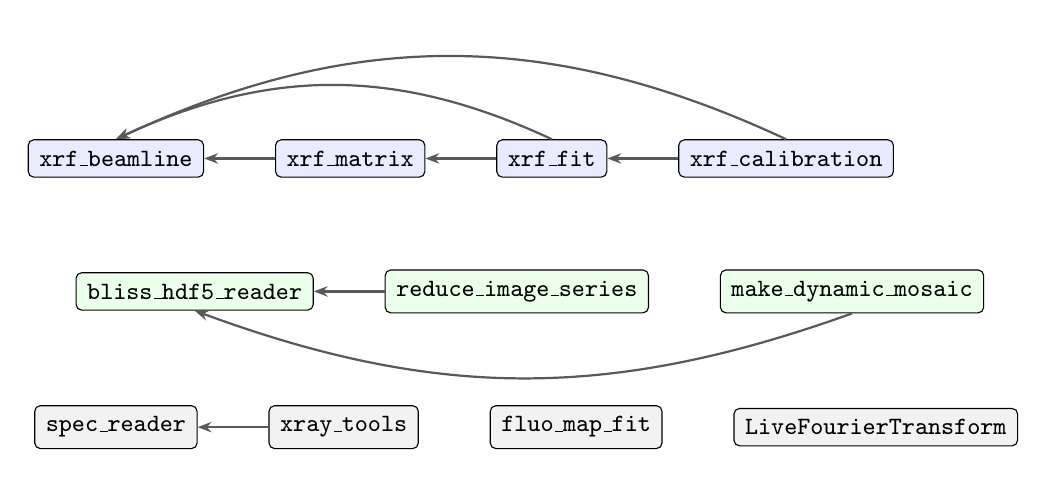
\begin{tikzpicture}[
  mod/.style={draw, rounded corners=2pt, font=\ttfamily\small, inner sep=4pt, fill=#1},
  mod/.default={white},
  dep/.style={-{Stealth[length=5pt]}, thick, gray!70!black},
  node distance=6mm and 9mm]
\node[mod=blue!8] (beam) {xrf\_beamline};
\node[mod=blue!8, right=of beam] (matrix) {xrf\_matrix};
\node[mod=blue!8, right=of matrix] (fit) {xrf\_fit};
\node[mod=blue!8, right=of fit] (cal) {xrf\_calibration};
\node[mod=green!8, below=12mm of beam, xshift=10mm] (bliss) {bliss\_hdf5\_reader};
\node[mod=green!8, right=of bliss] (red) {reduce\_image\_series};
\node[mod=green!8, right=of red] (mos) {make\_dynamic\_mosaic};
\node[mod=gray!10, below=12mm of bliss, xshift=-10mm] (spec) {spec\_reader};
\node[mod=gray!10, right=of spec] (xt) {xray\_tools};
\node[mod=gray!10, right=of xt] (fmf) {fluo\_map\_fit};
\node[mod=gray!10, right=of fmf] (lft) {LiveFourierTransform};
\draw[dep] (matrix) -- (beam);
\draw[dep] (fit) -- (matrix);
\draw[dep] (fit.north) to[bend right=25] (beam.north);
\draw[dep] (cal) -- (fit);
\draw[dep] (cal.north) to[bend right=25] (beam.north);
\draw[dep] (red) -- (bliss);
\draw[dep] (mos.south) to[bend left=20] (bliss.south);
\draw[dep] (xt) -- (spec);
\end{tikzpicture}
\caption{Imports between the modules (an arrow points to the module that is imported).
Blue: fluorescence analysis; green: BLISS data and diffraction images; grey: older or
superseded tools. The notebooks (Section~\ref{sec:notebooks}) sit on top of the blue modules
and of \fn{bliss_hdf5_reader}.}
\label{fig:deps}
\end{figure}

The physics of the fluorescence chain is explained, with figures from real BM32 data, in the
technical note \fn{docs/xrf_quantification/xrf_quantification.pdf}; this document is its
companion on the code side and repeats the equations where a function implements them.

\subsection{Dependencies}

\begin{description}[leftmargin=1.6em,itemsep=1pt,font=\normalfont\ttfamily]
\item[numpy, scipy] arrays, special functions (Bessel $K_\nu$, $\erfc$, $\erfcx$, Voigt),
quadrature, and the bounded non-linear least-squares solver of
\fn{scipy.optimize.curve_fit} (trust-region reflective algorithm
\citep{Branch1999,Virtanen2020}).
\item[xraylib] atomic and X-ray data \citep{Brunetti2004,Schoonjans2011}: line energies,
radiative rates, fluorescence yields, partial photo-ionisation cross-sections, the
``Kissel'' partial fluorescence cross-sections that include Coster--Kronig transfer,
attenuation coefficients of elements and compounds, refractive indices, and Hartree--Fock
Compton profiles \citep{Biggs1975}. Tested with xraylib 4.3.
\item[h5py] HDF5 files \citep{Collette2013}, including virtual datasets.
\item[matplotlib] plots (imported inside the plotting functions only).
\item[fabio, tqdm] TIFF images and progress bars in the image scripts.
\end{description}
The analysis environment used on the beamline runs Python~3.12, NumPy~2.5, SciPy~1.18,
xraylib~4.3 and h5py~3.16.

\subsection{Conventions}\label{sec:conventions}

\paragraph{Units.} The units are part of the argument names wherever a quantity has one
(\fn{energy_ev}, \fn{thickness_um}, \fn{air_path_cm}, \fn{grazing_angle_mrad} \dots).
The fluorescence fit works in \textbf{eV} (line energies, widths, calibration), while xraylib
and the beam and matrix modules work in \textbf{keV}; conversions are explicit in the code.
Mass attenuation coefficients and cross-sections are in cm$^2$/g, densities in g/cm$^3$, mass
thicknesses in g/cm$^2$. Angles of the sample geometry are in degrees from the sample
\emph{surface}; beamline angles are in mrad (mirrors) or \textmu rad (source acceptance).

\paragraph{Spectral flux.} Synchrotron fluxes are given, as is customary, per 0.1\,\%
bandwidth: $N_{0.1\%}(E)$ photons in the energy interval $\dd E = 10^{-3}E$. Integrals over
energy need the density per unit energy,
\begin{equation}
  \frac{\dd N}{\dd E} = \frac{N_{0.1\%}(E)}{10^{-3}\,E},
  \label{eq:per-energy}
\end{equation}
which \fn{xrf_beamline.per_unit_energy} implements and every function that integrates over the
incident spectrum applies internally. Forgetting this Jacobian over-weights high energies by
a factor $E$.

\paragraph{Channels and calibration.} MCA channels are numbered from 0. The energy
calibration is linear, $E = G\,c + O$ with gain $G$ (eV/channel) and offset $O$ (eV). Channel
ranges are half-open, $[c_\mathrm{lo}, c_\mathrm{hi})$, as Python slices.

\paragraph{Uncertainties.} All quoted errors are one standard deviation. Fit uncertainties
come from the covariance matrix of the linearised least-squares problem (Section~\ref{sec:fitting}).

\paragraph{Line names.} Fluorescence lines are named with IUPAC notation (initial vacancy,
final vacancy): \fn{KL3} is K$\alpha_1$, \fn{L3M5} is L$\alpha_1$, \fn{L2M4} L$\beta_1$,
\fn{L2N4} L$\gamma_1$, \fn{M5N7} M$\alpha_1$. Table~\ref{tab:siegbahn} in
Section~\ref{sec:calibration} gives the correspondence used for labels.

\subsection{How to read the function entries}

Each documented class or function has an entry with, in this order: what it does; its
arguments (name, type, default and meaning) and what it returns; the method, with the
equations it evaluates; its hypotheses and limits (blue boxes); known problems (red boxes);
the references; and the code. The listings are copied from the source files by
\fn{make_listings.py}, so the numbers in their margin are the line numbers of the file at
commit \sourceversion. Methods are shown without their class indentation. A class listing
contains the class header, its docstring and its fields; each method follows separately.
Private helpers (names starting with an underscore) are documented like public functions,
since they hold much of the physics.

%==========================================================================================
\section{\texttt{bliss\_hdf5\_reader}: reading BLISS scans}\label{sec:bliss}
%==========================================================================================

\subsection{Overview}

BLISS, the ESRF beamline control system, writes one HDF5 \emph{master file} per dataset,
organised along NeXus conventions \citep{Konnecke2015}. Every scan is an entry named
\fn{"<number>.<subscan>"} (\fn{"12.1"}) containing:
\begin{itemize}[nosep]
\item \fn{title}: the command as typed (\fn{"amesh xech 0 1 50 yech 0 1 40 0.1"}),
  \fn{start_time}, \fn{end_time}, \fn{end_reason} (\fn{SUCCESS}, \fn{USER_ABORT}, \dots);
\item \fn{measurement/}: one dataset per recorded quantity, one entry per scan point along
  the first axis (scalar counters and motor positions: shape $(n)$; MCA spectra:
  $(n, n_\mathrm{ch})$; detector images: $(n, h, w)$). These are links to the
  \fn{instrument/} group;
\item \fn{instrument/positioners_start}: every motor position at the start of the scan;
  \fn{instrument/<name>} groups with an \fn{NX_class} attribute (\fn{NXpositioner} for motors);
\item \fn{scan_parameters/}: \fn{npoints}, \fn{count_time} and other parameters, when recorded;
\item \fn{writer/status}, \fn{sample/name}.
\end{itemize}
Detector images are written by Lima in separate files of a \fn{scanNNNN/} folder next to the
master file; the master file exposes them as an HDF5 \emph{virtual dataset}, which maps
ranges of the virtual array onto datasets of the source files.

The module turns this into a \fn{BlissScan} object that knows the \emph{geometry} of the scan
(its shape in acquisition order, the motor driving each dimension, back-and-forth rows,
aborted points) and reads the data on demand. The geometry comes from parsing the command in
the title when it is recognised (Table~\ref{tab:bliss-titles}), and otherwise from the
recorded motor positions, so that scans run through user macros with custom titles are
still read correctly.

\begin{table}[h]
\centering\small
\caption{Scan commands recognised in titles, and the resulting shape (slowest axis first).}
\label{tab:bliss-titles}
\begin{tabularx}{\textwidth}{@{}l X l@{}}
\toprule
Command & Title grammar & Shape \\
\midrule
\fn{ascan dscan a2scan d3scan lineup} & $(\text{motor}\ \text{start}\ \text{stop})\times N$,
intervals, count time & $(\text{intervals}+1,)$ \\
\fn{amesh dmesh} & fast motor start stop intervals, slow motor start stop intervals, time
(the \emph{first} motor is the fast one) & $(n_\mathrm{slow}, n_\mathrm{fast})$ \\
\fn{fscan fscan2d fscan3d} & $(\text{motor}\ \text{start}\ \text{step}\ \text{npoints})\times
d$, acquisition time [period] (the \emph{last} motor is the fast one) & $(n_0,\dots,n_{d-1})$ \\
\texttt{f2scan f3scan \dots} & $(\text{motor}\ \text{start}\ \text{step})\times N$, npoints,
time & $(n,)$ \\
\fn{loopscan} & npoints, time & $(n,)$ \\
\fn{timescan ftimescan} & time [npoints] (0 or absent: until stopped) & $(n,)$ \\
\fn{ct sct} & [time] & $()$ \\
\bottomrule
\end{tabularx}
\end{table}

\begin{hyp}
\begin{itemize}[nosep,leftmargin=1em]
\item Data are stored in acquisition order, one entry per point along the first axis.
  Meshes are row-major with the slow motor first.
\item The number of recorded points is the most common first-axis length of the measurement
  datasets (fast scans add ``\fn{*_raw}'' channels with $2n+1$ entries, which are ignored).
\item A mesh scanned back and forth (snake) is recognised when the second row of the fast
  motor matches the reversed first row better than the first row itself.
\item An aborted 1D scan keeps its recorded length; an aborted mesh keeps its planned shape
  and missing points are NaN in gridded data.
\item Frames are read through the master file's virtual dataset; when there is none, the
  image files are found by listing the scan folder (top level only).
\end{itemize}
\end{hyp}

\subsection{Module header and helpers}

\pycode{bliss_hdf5_reader}{_header}

The constants list the positioner names that are time axes, not motors (\fn{TIME_AXES}),
the commands without a motor (\fn{TIME_SCANS}) and the single-point commands.

\api[\texttt{\_open}]{\texttt{\_open(path)}}
Opens a file read-only with HDF5 file locking disabled (\fn{locking=False}), so that a file
that BLISS is still writing can be read at the beamline; falls back to the default for
h5py older than 3.5, which has no \fn{locking} argument. Returns an \fn{h5py.File}, to be
used as a context manager.
\pycode{bliss_hdf5_reader}{_open}

\api[\texttt{\_to\_str}, \texttt{\_read\_scalar}, \texttt{\_is\_number}]{\texttt{\_to\_str(value)}, \texttt{\_read\_scalar(group, name)}, \texttt{\_is\_number(token)}}
\fn{_to_str} decodes bytes (UTF-8, with replacement of invalid sequences) and zero-dimensional
arrays to a Python string. \fn{_read_scalar} returns \fn{group[name]} as a Python scalar or
string, or \fn{None} if the dataset is missing. \fn{_is_number} tells whether a title token
parses as a float.
\pycode{bliss_hdf5_reader}{_to_str}
\pycode{bliss_hdf5_reader}{_read_scalar}
\pycode{bliss_hdf5_reader}{_is_number}

\api[\texttt{\_parse\_key}]{\texttt{\_parse\_key(scan, subscan)}}
Accepts a scan given as an integer (\fn{12}), a string (\fn{"12"}) or a full entry key
(\fn{"12.2"}). Returns \fn{(number, subscan, key)}; the subscan of a full key takes
precedence over the \fn{subscan} argument.
\pycode{bliss_hdf5_reader}{_parse_key}

\api[\texttt{list\_scans}]{\texttt{list\_scans(h5\_filepath)}}
Lists the scans of a master file without reading any data.
\blk{Returns} a list of dictionaries, one per top-level group, with keys \fn{key},
\fn{number} (integer part of the key, or \fn{None}), \fn{title}, \fn{npoints} (planned, from
\fn{scan_parameters}, if recorded), \fn{end_reason} and \fn{start_time}, sorted numerically by
scan then subscan (so \fn{"10.1"} comes after \fn{"9.1"}).
\pycode{bliss_hdf5_reader}{list_scans}

\api{\texttt{ScanMotor}}
A motor driven by the scan: \fn{name}, \fn{dim} (the scan dimension it drives, 0 = slowest),
\fn{npoints} along that dimension, \fn{start} and \fn{stop} as written in the title
(relative to the current position for d-scans, flagged by \fn{relative}). Its \fn{step}
property is $(\text{stop}-\text{start})/(n-1)$, or \fn{None} when undefined. Several motors can
share a dimension (\fn{a2scan}, the slow motors of an inferred mesh).
\pycode{bliss_hdf5_reader}{ScanMotor}
\pycode{bliss_hdf5_reader}{ScanMotor.step}

\api{\texttt{FrameSource}}
Location of one detector frame on disk: the source \fn{file}, the internal \fn{dataset}
path, and the frame \fn{index} in that dataset. Produced by \fn{BlissScan.frame_sources}.
\pycode{bliss_hdf5_reader}{FrameSource}

\subsection{Title parsers}

Each parser receives the command and the list of title tokens (commas are treated as
spaces) and returns \fn{(shape, motors, count_time)}, or \fn{None} if the tokens do not
follow the expected grammar---in which case the geometry is inferred from the data.

\api[\texttt{\_parse\_step\_scan}]{\texttt{\_parse\_step\_scan(cmd, args)}}
Step scans with $N$ motors: $3N+2$ tokens, each triple a motor name and two numbers, then an
integer number of intervals and a count time. The number of points is intervals $+1$.
Commands starting with \fn{d}, and \fn{lineup}, are relative.
\pycode{bliss_hdf5_reader}{_parse_step_scan}

\api[\texttt{\_parse\_mesh}]{\texttt{\_parse\_mesh(cmd, args)}}
\fn{amesh}/\fn{dmesh}: the first motor is the fast one, but the returned shape and motor
list put the slow motor first, so that every 2D scan has shape $(n_\mathrm{slow},
n_\mathrm{fast})$ whatever the command.
\pycode{bliss_hdf5_reader}{_parse_mesh}

\api[\texttt{\_parse\_fscan\_nd}]{\texttt{\_parse\_fscan\_nd(cmd, args)}}
Continuous scans \fn{fscan}, \fn{fscan2d}, \fn{fscan3d}: $d$ groups of (motor, start, step,
npoints), the \emph{last} motor being the fast one; the stop position is $\text{start} +
\text{step}\,(n-1)$.
\pycode{bliss_hdf5_reader}{_parse_fscan_nd}

\api[\texttt{\_parse\_fnscan}]{\texttt{\_parse\_fnscan(cmd, args)}}
Continuous scans of several motors along one dimension (\fn{f2scan}, \fn{f3scan}): the
number of motors is read from the command name.
\pycode{bliss_hdf5_reader}{_parse_fnscan}

\api[\texttt{\_parse\_time\_scan}, \texttt{\_parse\_single\_point}]{\texttt{\_parse\_time\_scan(cmd, args)}, \texttt{\_parse\_single\_point(cmd, args)}}
Scans without motors. A \fn{timescan} without a number of points runs until it is stopped:
its planned size is unknown (shape $(0,)$ at this stage, replaced by the recorded length).
\fn{ct}/\fn{sct} have shape $()$.
\pycode{bliss_hdf5_reader}{_parse_time_scan}
\pycode{bliss_hdf5_reader}{_parse_single_point}

\api[\texttt{\_parse\_title}]{\texttt{\_parse\_title(title)}}
Dispatches on the first token with regular expressions (\texttt{[ad]\textbackslash d*scan\textbar{}lineup},
\texttt{f\textbackslash d+scan}) and the command tables. Returns \fn{(command, parsed)} with \fn{parsed}
\fn{None} for unknown commands.
\pycode{bliss_hdf5_reader}{_parse_title}

\subsection{\texttt{BlissScan}}

\api[\texttt{BlissScan}]{\texttt{BlissScan(h5\_filepath, scan\_number, subscan=1, image\_prefix="eiger", image\_suffix=".h5", verbose=False)}}
One scan of a master file, of any type. Instantiation reads only metadata; data are read on
demand.
\begin{args}
\item[h5\_filepath] path of the master file.
\item[scan\_number] integer, or full key \fn{"12.1"}.
\item[subscan] used when \fn{scan_number} is an integer (default 1).
\item[image\_prefix] preferred image detector: the first image dataset whose name starts
  with it (default \fn{"eiger"}); \fn{None} takes the first image detector.
\item[image\_suffix] extension of image files when they have to be found by listing the
  scan folder.
\item[verbose] print the summary after \fn{read_data()}.
\end{args}
\blk{Main attributes} \fn{title}, \fn{command} (and its former name \fn{scan_type}),
\fn{shape}, \fn{motors} (list of \fn{ScanMotor}), \fn{npoints} (recorded),
\fn{npoints_planned}, \fn{count_time}, \fn{snake}, \fn{geometry_source} (\fn{"title"} or
\fn{"data"}), \fn{start_time}, \fn{end_time}, \fn{end_reason}, \fn{writer_status},
\fn{sample_name}, \fn{scan_folder}; after \fn{read_data()}: \fn{counters} (raw arrays),
\fn{grids} (scalar counters on the scan grid), \fn{image_path_list}, \fn{nb_images},
\fn{nb_frames}.
\pycode{bliss_hdf5_reader}{BlissScan}
\pycode{bliss_hdf5_reader}{BlissScan.__init__}

\api[\texttt{BlissScan.\_read\_metadata}]{\texttt{BlissScan.\_read\_metadata()}}
The core of the reader. It opens the file once and reads the entry's scalars, the shapes and
types of every measurement dataset (not the data), the positioner names
(\fn{_find_positioners}), the number of recorded points (\fn{_count_acquired_points}) and the
positions of every positioner recorded once per point (kept in a cache for geometry
inference and snake detection). It then:
\begin{enumerate}[nosep]
\item parses the title; if that fails, infers the geometry from the motor positions;
\item takes the count time from \fn{scan_parameters}, else from the title;
\item determines the planned number of points: the product of the title shape, overridden
  by \fn{scan_parameters/npoints} if they disagree (with a warning);
\item for 0D and 1D scans, replaces the shape by what was recorded;
\item detects back-and-forth meshes.
\end{enumerate}
Raises \fn{FileNotFoundError} or \fn{KeyError} if the file or the scan does not exist.
\pycode{bliss_hdf5_reader}{BlissScan._read_metadata}

\api[\texttt{BlissScan.\_find\_positioners}]{\texttt{BlissScan.\_find\_positioners(entry, meas)} (static)}
Motors among the measurement datasets: names present in \fn{positioners_start}, and datasets
whose link target is an \fn{instrument/} group of class \fn{NXpositioner}. The second rule
catches the fast motor of continuous scans, recorded as an encoder channel. Time axes are
excluded.
\pycode{bliss_hdf5_reader}{BlissScan._find_positioners}

\api[\texttt{BlissScan.\_count\_acquired\_points}]{\texttt{BlissScan.\_count\_acquired\_points(npts\_param)}}
The number of recorded points is the most common first-dimension length among the
measurement datasets (ties broken towards the larger value). Lengths above the planned number
of points are discarded first, which removes the $2n+1$ ``\fn{*_raw}'' channels of fast
scans.
\pycode{bliss_hdf5_reader}{BlissScan._count_acquired_points}

\api[\texttt{BlissScan.\_infer\_geometry}]{\texttt{BlissScan.\_infer\_geometry(npts\_planned=None)}}
Geometry for unrecognised titles. Motors that do not move (peak-to-peak range below
$10^{-9}$ of their magnitude) are ignored. If the moving motors form a mesh
(\fn{_infer_mesh}), the shape is $(n_\mathrm{slow}, n_\mathrm{fast})$, extended to the planned
number of rows for an aborted mesh; otherwise the scan is 1D and every moving motor drives
dimension 0.
\pycode{bliss_hdf5_reader}{BlissScan._infer_geometry}

\api[\texttt{BlissScan.\_row\_length}]{\texttt{BlissScan.\_row\_length(pos)} (static)}
Tests whether a position series is the slow motor of a mesh: it must jump at regular
intervals (one jump per row, all rows of equal length, at least two full rows) and stay
constant within a row (range within a row below a tenth of the median jump). Returns the row
length or \fn{None}.
\pycode{bliss_hdf5_reader}{BlissScan._row_length}

\api[\texttt{BlissScan.\_infer\_mesh}]{\texttt{BlissScan.\_infer\_mesh(moving)} (class method)}
For each candidate row length (shortest first), the slow motors are those with that row
length, and the fast motors those that repeat the same positions on the second row as on
the first, in the same or the reversed order (mismatch below a tenth of their range).
Returns \fn{((n_slow, n_fast), motors)} or \fn{None}.
\pycode{bliss_hdf5_reader}{BlissScan._infer_mesh}

\api[\texttt{BlissScan.\_detect\_snake}]{\texttt{BlissScan.\_detect\_snake()}}
A 2D scan is back-and-forth if the second row of the fast motor is closer to the reversed
first row than to the first row itself.
\pycode{bliss_hdf5_reader}{BlissScan._detect_snake}

\api[Properties: \texttt{ndim}, \texttt{is\_complete}, \texttt{motor\_names}, \texttt{positioner\_names}; \texttt{motors\_of\_dim}]{Properties: \texttt{ndim}, \texttt{is\_complete}, \texttt{motor\_names}, \texttt{positioner\_names}; \texttt{motors\_of\_dim(dim)}}
\fn{is_complete} is \fn{end_reason == "SUCCESS"} when the end reason is recorded, otherwise
a comparison of recorded and planned points. \fn{positioner_names} lists every motor
recorded at each point, scanned or not.
\pycode{bliss_hdf5_reader}{BlissScan.ndim}
\pycode{bliss_hdf5_reader}{BlissScan.is_complete}
\pycode{bliss_hdf5_reader}{BlissScan.motor_names}
\pycode{bliss_hdf5_reader}{BlissScan.positioner_names}
\pycode{bliss_hdf5_reader}{BlissScan.motors_of_dim}

\api[\texttt{BlissScan.index\_grid}]{\texttt{BlissScan.index\_grid} (property)}
The flat point index at each grid position, $-1$ where no point was recorded; odd rows are
reversed for a back-and-forth mesh. It is the single object that places per-point data on
the grid, used by \fn{to_grid} and by the image scripts.
\pycode{bliss_hdf5_reader}{BlissScan.index_grid}

\api[\texttt{get\_available\_counters}, \texttt{get}, \texttt{\_\_getitem\_\_}, \texttt{positions}]{\texttt{get\_available\_counters()} (alias \texttt{list\_counters}), \texttt{get(name, grid=False)}, \texttt{\_\_getitem\_\_(name)}, \texttt{positions(motor, grid=False)}}
\fn{get_available_counters} returns \texttt{\{name: \{"shape", "dtype"\}\}} for every
measurement dataset without reading data. \fn{get} reads one dataset (or returns it from
\fn{counters} if \fn{read_data} loaded it), warns when it would load more than 2\,GB, and
with \fn{grid=True} reshapes the point axis to the scan shape: an MCA dataset of a mesh
becomes $(n_\mathrm{slow}, n_\mathrm{fast}, n_\mathrm{ch})$. \fn{scan["name"]} is
\fn{get(name, grid=True)}; \fn{positions} returns floats.
\pycode{bliss_hdf5_reader}{BlissScan.get_available_counters}
\pycode{bliss_hdf5_reader}{BlissScan.get}
\pycode{bliss_hdf5_reader}{BlissScan.__getitem__}
\pycode{bliss_hdf5_reader}{BlissScan.positions}

\api[\texttt{BlissScan.to\_grid}]{\texttt{BlissScan.to\_grid(data, name="array")}}
Places per-point data on the scan grid. Complete, non-snake data are simply reshaped. With
missing points (aborted mesh) the output is filled with NaN (integer data are promoted to
floating point for that) and the recorded points are placed through \fn{index_grid}, which
also un-snakes back-and-forth rows. A counter with one value more than the grid (BLISS
sometimes records one point ahead on abort) is truncated. Raises \fn{ValueError} when the
first axis is not one value per point.
\pycode{bliss_hdf5_reader}{BlissScan.to_grid}

\api[\texttt{BlissScan.read\_data}]{\texttt{BlissScan.read\_data(extra\_counters=None)}}
Loads the scanned motors and the requested counters into \fn{counters}, grids every 1D
counter into \fn{grids}, and locates the image files (\fn{_process_images}). Missing names
produce warnings, not errors.
\pycode{bliss_hdf5_reader}{BlissScan.read_data}

\subsection{Detector frames}

\api[\texttt{image\_detectors}, \texttt{spectrum\_detectors} ; \texttt{\_pick\_detector}]{\texttt{image\_detectors}, \texttt{spectrum\_detectors} (properties); \texttt{\_pick\_detector(detector)}}
Datasets with one 2D image per point (3D datasets) and with one spectrum per point (2D
datasets). \fn{_pick_detector} returns the named detector, or the first image detector
matching \fn{image_prefix}, or the first image detector.
\pycode{bliss_hdf5_reader}{BlissScan.image_detectors}
\pycode{bliss_hdf5_reader}{BlissScan.spectrum_detectors}
\pycode{bliss_hdf5_reader}{BlissScan._pick_detector}

\api[\texttt{BlissScan.frame\_sources}]{\texttt{BlissScan.frame\_sources(detector=None)}}
Reads the mapping of the virtual dataset: for each virtual source, the selection bounds in
the virtual and source spaces give the range of frames it holds; relative file names are
resolved against the master file's folder. Returns one \fn{FrameSource} per frame, or an
empty list when the detector is not a virtual dataset.
\pycode{bliss_hdf5_reader}{BlissScan.frame_sources}

\api[\texttt{read\_frame}, \texttt{iter\_frames}]{\texttt{read\_frame(index, detector=None, roi=None)}, \texttt{iter\_frames(detector=None, indices=None, roi=None)}}
One frame by point index, read through the master file (HDF5 resolves the virtual mapping),
optionally restricted to \fn{roi = (row slice, column slice)} so that only that part is read
from disk. \fn{iter_frames} yields frames while keeping the file open, which is much faster
than repeated \fn{read_frame} calls.
\pycode{bliss_hdf5_reader}{BlissScan.read_frame}
\pycode{bliss_hdf5_reader}{BlissScan.iter_frames}

\api[\texttt{BlissScan.\_process\_images}]{\texttt{BlissScan.\_process\_images()}}
Fills \fn{image_path_list} with the distinct image files in acquisition order (from the
virtual dataset, or by listing \fn{scanNNNN/<prefix>*<suffix>}), \fn{nb_images} (files) and
\fn{nb_frames} (frames).
\pycode{bliss_hdf5_reader}{BlissScan._process_images}

\subsection{Other methods, the mesh subclass and the command line}

\api[\texttt{positioners\_start}, \texttt{get\_relative\_position\_grid}, \texttt{summary}, \texttt{get\_summary}, \texttt{\_\_repr\_\_}]{\texttt{positioners\_start()}, \texttt{get\_relative\_position\_grid(motor\_name, scale=1000.0)}, \texttt{summary()}, \texttt{get\_summary()}, \texttt{\_\_repr\_\_()}}
\fn{positioners_start} returns the snapshot of every motor at the start of the scan.
\fn{get_relative_position_grid} returns the gridded positions minus that of the first
recorded point, times \fn{scale} (mm to \textmu m by default). \fn{summary} is a
human-readable description: shape and its source, points recorded and planned, completion,
snake, count time, motors with their ranges and steps, detectors, loaded counters.
\pycode{bliss_hdf5_reader}{BlissScan.positioners_start}
\pycode{bliss_hdf5_reader}{BlissScan.get_relative_position_grid}
\pycode{bliss_hdf5_reader}{BlissScan.summary}
\pycode{bliss_hdf5_reader}{BlissScan.get_summary}
\pycode{bliss_hdf5_reader}{BlissScan.__repr__}

\api{\texttt{BlissMeshScan}}
A \fn{BlissScan} that must be two-dimensional (\fn{ValueError} otherwise), kept for scripts
written for the former mesh-only reader. It adds the attributes \fn{slow_/fast_motor_name},
\fn{_start}, \fn{_stop}, \fn{_steps}, \fn{_intervals}, \fn{_step_size}, \fn{scan_shape} and
\fn{expected_points}.
\pycode{bliss_hdf5_reader}{BlissMeshScan}
\pycode{bliss_hdf5_reader}{BlissMeshScan._read_metadata}

\api[\texttt{main}]{\texttt{main()}}
Command line: \fn{python bliss_hdf5_reader.py file.h5} lists the scans (key, planned
points, end reason, title); with scan keys after the file name it prints their summaries and
dataset shapes.
\pycode{bliss_hdf5_reader}{main}

%==========================================================================================
\section{\texttt{xrf\_beamline}: the incident spectrum}\label{sec:beamline}
%==========================================================================================

\subsection{Overview}

Under white-beam (Laue) illumination every element is excited by the whole incident
spectrum $\Phi(E)$, and the relative intensities of its fluorescence lines---not only its
total signal---depend on the shape of that spectrum: each L or M subshell is ionised only by
photons above its own edge, and those edges can be kilo-electronvolts apart (Ir: L$_3$ at
11.22\,keV, L$_1$ at 13.42\,keV). The module computes $\Phi(E)$ at the sample from first
principles: the synchrotron radiation of a bending magnet \citep{Schwinger1949,Kim1989},
accepted through the apertures of the beamline, and filtered by grazing-incidence mirrors
\citep{Parratt1954,Nevot1980}, beryllium windows and the air path. It also provides narrow
``monochromatic'' spectra for tube or monochromator excitation, and the air model used by
the detector-efficiency calculation of \fn{xrf_fit}.

The quantities returned by \fn{Beamline.spectrum} are fluxes per mrad of horizontal angle
and per 0.1\,\% bandwidth; only their \emph{shape} matters for line ratios and for the
matrix corrections, but the absolute scale is correct (photons/s) for a given ring current.

\begin{hyp}
\begin{itemize}[nosep,leftmargin=1em]
\item Bending-magnet radiation of a filament electron beam (no emittance, no energy spread);
  the horizontal fan is uniform, so horizontal apertures scale the flux but not the spectrum.
\item Mirrors: specular s-polarised Fresnel reflectivity of a homogeneous coating of nominal
  density, with an optional N\'evot--Croce roughness factor; no slope errors, no thermal
  deformation, no contamination layer. Bent mirrors act as thin cylindrical lenses in the
  paraxial approximation.
\item Windows and air: Beer--Lambert attenuation with total cross-sections; dry air, ideal
  gas.
\item The BM32 defaults (magnetic field 0.86\,T, Ir coatings, $2\times500$\,\textmu m Be,
  3.3\,m of air, element positions) were confirmed in October 2026; mirror roughness is
  unknown (0) and the KB grazing angles are not recorded in the scan files (3\,mrad).
\end{itemize}
\end{hyp}

\pycode{xrf_beamline}{_header}

\subsection{Source}

\api[\texttt{BendingMagnetSource}]{\texttt{BendingMagnetSource(ring\_energy\_gev=6.04, magnetic\_field\_t=0.86, current\_a=0.2)}}
Synchrotron radiation of a bending magnet. The defaults describe the BM32 source on ESRF-EBS.
\begin{args}
\item[ring\_energy\_gev] electron energy $E_e$ (6.04\,GeV for EBS).
\item[magnetic\_field\_t] dipole field $B$; sets the critical energy, to which the high-energy
  end of the spectrum is exponentially sensitive.
\item[current\_a] ring current $I$, in amperes.
\end{args}
\blk{Physics} The critical energy and the Lorentz factor are
\begin{equation}
  E_c\,[\mathrm{keV}] = 0.665\,E_e^2[\mathrm{GeV}]\,B[\mathrm{T}], \qquad
  \gamma = \frac{E_e}{m_e c^2} \approx 11\,820 ,
\end{equation}
giving $E_c = 20.9$\,keV for BM32. With $y = E/E_c$, the flux integrated over the vertical
opening angle, per mrad of horizontal angle and per 0.1\,\% bandwidth, is \citep{Kim1989}
\begin{equation}
  \frac{\dd N}{\dd\theta} = 2.457\times10^{13}\,E_e[\mathrm{GeV}]\,I[\mathrm{A}]\;G_1(y),
  \qquad G_1(y) = y\int_y^\infty K_{5/3}(x)\,\dd x ,
  \label{eq:g1}
\end{equation}
and the angular density at vertical angle $\psi$, per mrad$^2$, with $X = \gamma\psi$ and
$\xi = \tfrac{y}{2}(1+X^2)^{3/2}$, is
\begin{equation}
  \frac{\dd^2 N}{\dd\theta\,\dd\psi} = 1.327\times10^{13}\,E_e^2\,I\;y^2(1+X^2)^2
  \left[K_{2/3}^2(\xi) + \frac{X^2}{1+X^2}K_{1/3}^2(\xi)\right],
  \label{eq:angular}
\end{equation}
where the first term is the horizontally ($\sigma$) polarised part and the second the
vertically ($\pi$) polarised part. On axis it reduces to $1.327\times10^{13}E_e^2 I\,H_2(y)$
with $H_2(y) = y^2K_{2/3}^2(y/2)$. The vertical opening angle is of order $1/\gamma =
85$\,\textmu rad, and wider for soft photons, so an aperture that accepts only a few
\textmu rad selects the harder on-axis spectrum.
\pycode{xrf_beamline}{BendingMagnetSource}

\api[\texttt{critical\_energy\_kev}, \texttt{gamma} ; \texttt{\_g1}]{\texttt{critical\_energy\_kev}, \texttt{gamma} (properties); \texttt{\_g1(y)} (static)}
$E_c$ and $\gamma$ as above. \fn{_g1} evaluates $G_1(y)$ by adaptive quadrature of
$K_{5/3}$ (\fn{scipy.special.kv}) from $y$ to infinity; it returns 0 for $y\le0$ and for
$y>50$, where $G_1 < 10^{-20}$.
\pycode{xrf_beamline}{BendingMagnetSource.critical_energy_kev}
\pycode{xrf_beamline}{BendingMagnetSource.gamma}
\pycode{xrf_beamline}{BendingMagnetSource._g1}

\api[\texttt{spectral\_flux}]{\texttt{spectral\_flux(energies\_kev)}}
Eq.~\eqref{eq:g1} on an energy grid (keV): photons/s/mrad(horizontal)/0.1\,\%\,BW, integrated
over the vertical angle. Returns an array of the grid's size.
\pycode{xrf_beamline}{BendingMagnetSource.spectral_flux}

\api[\texttt{angular\_flux}]{\texttt{angular\_flux(energies\_kev, psi\_urad)}}
Eq.~\eqref{eq:angular}: photons/s/mrad$^2$/0.1\,\%\,BW, both polarisations, on a grid of
energies and vertical angles (\textmu rad). Returns an array of shape $(n_E, n_\psi)$.
Bessel functions that overflow or underflow far from the axis are set to zero.
\pycode{xrf_beamline}{BendingMagnetSource.angular_flux}

\api[\texttt{accepted\_flux}]{\texttt{accepted\_flux(energies\_kev, vertical\_acceptance\_urad=None, vertical\_offset\_urad=0.0, n\_angles=41)}}
Flux per mrad (horizontal) per 0.1\,\%\,BW inside the vertical window
$\psi_0 \pm \Delta\psi/2$: the trapezoidal integral of Eq.~\eqref{eq:angular} over
\fn{n_angles} angles, converted from \textmu rad to mrad. \fn{None} (or a non-finite value)
returns the full integral, Eq.~\eqref{eq:g1}. For $\Delta\psi \ll 1/\gamma$ the result is the
on-axis spectrum times $\Delta\psi$.
\pycode{xrf_beamline}{BendingMagnetSource.accepted_flux}

\subsection{Optical elements}

\api[\texttt{Mirror}]{\texttt{Mirror(material, density\_g\_cm3, grazing\_angle\_mrad, roughness\_nm=0.0, label="", distance\_m=None, length\_m=None, plane="vertical", bending\_radius\_m=inf, image\_distance\_m=None, angle\_spread\_mrad=0.0)}}
A grazing-incidence mirror. Its spectral effect is the reflectivity; if it is positioned
(\fn{distance_m} and \fn{length_m}), its footprint also acts as an aperture; if it is bent,
it focuses the beam divergence; if it is a focusing (KB) mirror, its grazing angle varies
along the footprint.
\begin{args}
\item[material, density\_g\_cm3] coating, e.g. \fn{"Ir"}, 22.56.
\item[grazing\_angle\_mrad] angle between the beam and the surface, $\theta$.
\item[roughness\_nm] r.m.s. roughness $\sigma$ (N\'evot--Croce factor; 0 disables it).
\item[distance\_m, length\_m] distance from the source and optical length.
\item[plane] \fn{"vertical"} or \fn{"horizontal"}: deflection plane.
\item[bending\_radius\_m] meridional radius $R$ (\fn{inf} for a flat mirror).
\item[image\_distance\_m] distance $q$ to the focus of a focusing mirror.
\item[angle\_spread\_mrad] half-range of grazing angles over the illuminated footprint;
  filled in by \fn{Beamline.resolved_optics} from \fn{image_distance_m}.
\end{args}
\pycode{xrf_beamline}{Mirror}
\pycode{xrf_beamline}{Mirror.__post_init__}

\api[\texttt{focal\_length\_m}, \texttt{aperture\_m}]{\texttt{focal\_length\_m}, \texttt{aperture\_m} (properties)}
A cylindrically bent mirror of radius $R$ at grazing angle $\theta$ focuses in its
deflection plane with focal length $f = R\sin\theta/2$ (the meridional Coddington equation
at grazing incidence). The footprint of length $L$ accepts a beam of size $L\sin\theta$.
\pycode{xrf_beamline}{Mirror.focal_length_m}
\pycode{xrf_beamline}{Mirror.aperture_m}

\api[\texttt{Mirror.transfer}, \texttt{Mirror.\_reflectivity}]{\texttt{Mirror.transfer(energies\_kev)}, \texttt{Mirror.\_reflectivity(energies\_kev, angle\_mrad)}}
\blk{Physics} With the complex refractive index $n = 1-\delta+i\beta$ of the coating (xraylib
\fn{Refractive_Index_Re} and \fn{_Im}), the s-polarised Fresnel amplitude at grazing angle
$\theta$ is \citep{Parratt1954,AlsNielsen2011}
\begin{equation}
  r_s = \frac{\sin\theta - q}{\sin\theta + q}, \qquad q = \sqrt{n^2-\cos^2\theta},
  \qquad R = |r_s|^2 .
\end{equation}
Total external reflection holds below the critical angle $\theta_c \approx \sqrt{2\delta}$;
since $\delta\propto E^{-2}$, a mirror at fixed angle cuts off above $E_c^\mathrm{mirror}
\propto 1/\theta$ (for Ir, $\delta = 3.4\times10^{-5}$ at 10\,keV, so $\theta_c = 8.3$\,mrad at
10\,keV and the edge of reflection at 3\,mrad lies near 27\,keV). Roughness multiplies the
\emph{amplitude} by $\exp(-2k_{z0}k_{z1}\sigma^2)$ \citep{Nevot1980}, with $k_{z0} =
k_0\sin\theta$ and $k_{z1} = k_0 q$, so the intensity factor is
$\exp(-4k_0^2\sin\theta\,\Re(q)\,\sigma^2)$; below the critical angle $\Re q \ll \sin\theta$
and the factor tends to 1, while well above it the Debye--Waller form
$\exp(-4k_{z0}^2\sigma^2)$ is recovered. Synchrotron radiation is polarised in the orbit
plane and the mirrors of BM32 deflect vertically, so s-polarisation is the relevant case
(at mrad angles both polarisations give the same result anyway).

\fn{transfer} returns $R(E)$, averaged uniformly over 21 angles in $\theta \pm$
\fn{angle_spread_mrad} if a spread is set. Energies where xraylib has no data get $n=1$.
\pycode{xrf_beamline}{Mirror.transfer}
\pycode{xrf_beamline}{Mirror._reflectivity}

\api[\texttt{Filter}; \texttt{transfer}]{\texttt{Filter(material, density\_g\_cm3, thickness\_um, label="")}; \texttt{transfer(energies\_kev)}}
A slab (window, filter, air path) with Beer--Lambert transmission
$T(E) = \exp[-(\mu/\rho)(E)\,\rho\,t]$, using the total mass attenuation coefficient of the
compound (\fn{CS_Total_CP}: photoabsorption plus coherent and incoherent scattering, since any
interaction removes the photon from the beam). Energies without data are fully absorbed.
\pycode{xrf_beamline}{Filter}
\pycode{xrf_beamline}{Filter.__post_init__}
\pycode{xrf_beamline}{Filter.transfer}

\api[\texttt{Slit}; \texttt{transfer}]{\texttt{Slit(distance\_m, vertical\_gap\_mm=None, horizontal\_gap\_mm=None, label="")}; \texttt{transfer}}
A pair of slits: an aperture without spectral effect (\fn{transfer} returns ones). A gap of
\fn{None} is open.
\pycode{xrf_beamline}{Slit}
\pycode{xrf_beamline}{Slit.__post_init__}
\pycode{xrf_beamline}{Slit.transfer}

\subsection{Monochromatic sources and units}

\api[\texttt{tube\_lines}]{\texttt{tube\_lines(anode, lines=("KL3", "KL2"))}}
Energies (eV) and relative intensities of X-ray tube anode lines, by default the K$\alpha_1$/
K$\alpha_2$ doublet that a crystal or multilayer monochromator passes (\fn{tube_lines("Mo")}:
17\,479 and 17\,374\,eV). The intensities are the radiative rates (\fn{RadRate}), normalised
to sum 1; this is correct for lines that share the same initial vacancy, such as K$\alpha_1$
and K$\alpha_2$. The constant \fn{OpticalElement}, the union type of the optics, precedes it
in the file.
\begin{hyp}
The monochromator passes both lines with the same efficiency and suppresses K$\beta$ and the
bremsstrahlung completely.
\end{hyp}
\pycode{xrf_beamline}{tube_lines}

\api[\texttt{monochromatic\_spectrum}]{\texttt{monochromatic\_spectrum(energies\_ev, weights=(1.0,), width\_ev=5.0, step\_ev=1.0)}}
Builds a narrow incident spectrum from Gaussian lines of standard deviation \fn{width_ev},
for the functions that expect an incident spectrum (\fn{element_line_groups},
\fn{MatrixModel}). The density per eV, normalised so that each line has area $w_i$, is
converted to the per-0.1\,\% bandwidth convention, $N_{0.1\%} = 10^{-3}E\,\dd N/\dd E$.
\blk{Returns} \texttt{(energy\_kev, flux\_per\_0.1\%BW)} on a grid from $8\sigma$ below the lowest to
$8\sigma$ above the highest line.
\begin{hyp}
The width only has to be resolved by the grid; its value does not matter as long as the
cross-sections vary slowly across it (true away from absorption edges). With
\fn{MatrixModel}, pass \fn{sf_step_kev = step_ev/1000}: its secondary-fluorescence grid is
decimated to 40\,eV by default, which would miss a 5\,eV-wide line.
\end{hyp}
\pycode{xrf_beamline}{monochromatic_spectrum}

\api[\texttt{per\_unit\_energy}]{\texttt{per\_unit\_energy(energies\_kev, flux\_01bw)}}
Eq.~\eqref{eq:per-energy}: per-0.1\,\% bandwidth flux to a density per keV. Integrals over
$\dd E$ (flux-weighted cross-sections) must use this form.
\pycode{xrf_beamline}{per_unit_energy}

\subsection{Air}

\api[\texttt{AIR\_FORMULA}, \texttt{air\_density}]{\texttt{AIR\_FORMULA}, \texttt{air\_density(temperature\_c=20.0, pressure\_hpa=1013.25)}}
Dry air is written as an atom-count formula from its volume composition (N$_2$ 78.084\,\%,
O$_2$ 20.946\,\%, Ar 0.934\,\%, CO$_2$ 0.0417\,\%): $\mathrm{N}_{156.168}\mathrm{O}_{41.975}
\mathrm{Ar}_{0.934}\mathrm{C}_{0.0417}$ per 100 molecules, which reproduces the mass fractions
N 75.5\,\%, O 23.2\,\%, Ar 1.29\,\%. Its density follows the ideal-gas law,
\begin{equation}
  \rho = \frac{P\,M}{R\,T}, \qquad M = 28.9647\ \mathrm{g/mol},
\end{equation}
returned in g/cm$^3$ (1.204\,mg/cm$^3$ at 20\,\textdegree C and 1013.25\,hPa).
\begin{hyp}
Humidity is neglected. Moist air is slightly lighter than dry air, so at 50\,\% relative
humidity and 20\,\textdegree C this overestimates density and absorption by a few parts per
thousand \citep{Picard2008}. The pressure is the local value: about 990\,hPa at the ESRF,
2.5\,\% below the sea-level standard.
\end{hyp}
\pycode{xrf_beamline}{air_density}

\api[\texttt{air\_path}]{\texttt{air\_path(length\_m, temperature\_c=20.0, pressure\_hpa=1013.25)}}
A \fn{Filter} of air of the given length. A long air path is the strongest low-energy filter
of a white-beam line: 3\,m transmit about $10^{-7}$ at 5\,keV, 1.7\,\% at 8\,keV and 12\,\% at
10\,keV.
\pycode{xrf_beamline}{air_path}

\subsection{The assembled beamline}

\api[\texttt{Beamline}]{\texttt{Beamline(source, optics=[], sample\_distance\_m=None, vertical\_acceptance="auto", vertical\_offset\_urad=0.0, settings=\{\})}}
A source and a list of optical elements. The elements with a position act as apertures
(slits through their gaps, mirrors through their footprint); \fn{acceptance} maps each of them
back to an angle at the source, and the smallest vertical one sets the window of source
angles whose spectrum is used.
\begin{args}
\item[source] a \fn{BendingMagnetSource}.
\item[optics] mirrors, filters and slits. Positions come from \fn{distance_m}; the order of
  the list only sets the order of labels and transfers.
\item[sample\_distance\_m] source--sample distance (for \fn{trace} and \fn{describe}).
\item[vertical\_acceptance] \fn{"auto"} (from the apertures), \fn{"full"} (vertically
  integrated spectrum, Eq.~\eqref{eq:g1}) or a number (full acceptance in \textmu rad).
\item[vertical\_offset\_urad] centre of the accepted window relative to the orbit plane.
\item[settings] free-form provenance (motor positions read from a scan).
\end{args}
\pycode{xrf_beamline}{Beamline}

\api[\texttt{\_positioned}, \texttt{trace}]{\texttt{\_positioned()}, \texttt{trace(plane="vertical")}}
Paraxial ray tracing. A ray leaves the source on axis with unit angle; at each positioned
element its height $h$ (per radian of source angle, in m/rad) is accumulated, and every
mirror bent in \fn{plane} changes the ray angle by $-h/f$ (thin concave lens). Returns
\fn{[(element, h), ...]} in order of distance, plus \fn{(None, h_sample)} if the sample
distance is set. The height per unit source angle is what converts an aperture into an
angular acceptance at the source.
\pycode{xrf_beamline}{Beamline._positioned}
\pycode{xrf_beamline}{Beamline.trace}

\api[\texttt{acceptance}]{\texttt{acceptance()}}
For each plane and each aperture, the full angular acceptance at the source in \textmu rad,
$\Delta\psi = s/h$ with $s$ the gap or the mirror's $L\sin\theta$. Returns
\texttt{\{"vertical": \{limits, acceptance\_urad, limited\_by\}, "horizontal": \{...\}\}}, with
infinite acceptance when nothing limits a plane.
\pycode{xrf_beamline}{Beamline.acceptance}

\api[\texttt{effective\_vertical\_acceptance}]{\texttt{effective\_vertical\_acceptance()}}
The acceptance actually used for the spectrum: \fn{None} for \fn{"full"} or when no aperture
limits the beam, the computed value for \fn{"auto"}, or the number given.
\pycode{xrf_beamline}{Beamline.effective_vertical_acceptance}

\api[\texttt{resolved\_optics}]{\texttt{resolved\_optics()}}
Returns the optics with the grazing-angle spread of each focusing mirror filled in. An
elliptical mirror receives nearly parallel rays from the distant source and sends them
converging to the focus at distance $q$; across an illuminated beam of size $s$ the outgoing
direction varies by $s/q$, so the grazing angle varies by
\begin{equation}
  \Delta\theta = \pm\frac{s}{4q}
\end{equation}
\citep{Kirkpatrick1948}. $s$ is the accepted angle in the mirror's plane times the height per
angle at the mirror, capped by the mirror's own aperture. The reflectivity is then averaged
over this range, which smooths the high-energy cut-off.
\pycode{xrf_beamline}{Beamline.resolved_optics}

\api[\texttt{describe}]{\texttt{describe()}}
A dictionary summarising the geometry: vertical and horizontal acceptances and the aperture
limiting each, every aperture's limit, the KB angle spreads, the height per \textmu rad at
each element, the acceptance and offset used.
\pycode{xrf_beamline}{Beamline.describe}

\api[\texttt{spectrum}, \texttt{spectral\_density}, \texttt{band\_limits}]{\texttt{spectrum(energies\_kev)}, \texttt{spectral\_density(energies\_kev)}, \texttt{band\_limits(energies\_kev, frac=0.01)}}
\fn{spectrum} returns \fn{(raw, transmitted, transfers)}: the accepted source flux, the flux at
the sample (the product of every mirror and filter transfer), and the list of
\fn{(label, transfer)}, all per mrad and per 0.1\,\%\,BW. \fn{spectral_density} converts the
transmitted flux to photons/s/mrad/keV. \fn{band_limits} gives the energies where the
transmitted flux first and last exceeds \fn{frac} of its maximum---a compact statement of the
usable band (about 5--25\,keV on BM32).
\pycode{xrf_beamline}{Beamline.spectrum}
\pycode{xrf_beamline}{Beamline.spectral_density}
\pycode{xrf_beamline}{Beamline.band_limits}

\subsection{BM32}

\api[\texttt{BM32\_LAYOUT}, \texttt{BM32\_WHITE\_BEAM}]{\texttt{BM32\_LAYOUT}, \texttt{BM32\_WHITE\_BEAM(air\_path\_m=3.3, temperature\_c=20.0, pressure\_hpa=1013.25, current\_a=0.2, magnetic\_field\_t=0.86, *, vg1=0.3, hg1=0.2, vg2=None, hg2=None, vg3=0.2, hg3=0.2, m1\_angle\_mrad=3.062, m2\_angle\_mrad=2.551, m1\_radius\_km=71.4, m2\_radius\_km=145.7, kbv\_angle\_mrad=3.0, kbh\_angle\_mrad=3.0, kb\_angle\_spread=True, vertical\_acceptance="auto", vertical\_offset\_urad=0.0)}}
The BM32 white-beam model. \fn{BM32_LAYOUT} holds the distances from the source (m) of the
primary slits s1 (26.368), the bent Ir mirrors m1 (28.309) and m2 (31.732), the guard slits s2
(35.370), the slits s3 that define the KB illumination (44.485), the KB mirrors (vertical
44.645, horizontal 44.880) and the sample (45.0), and the mirror lengths. The function builds:
s1; m1 and m2 (Ir, 22.56\,g/cm$^3$, bent); two 500\,\textmu m Be windows; s2; s3; KB-V and KB-H
(Ir, focusing, with angle spread if \fn{kb_angle_spread}); and the incident air path.
\begin{args}
\item[air\_path\_m] incident air path (3.3\,m measured on BM32); 0 removes it. Not to be
  confused with the sample--detector path of the detector model.
\item[vg1 \dots\ hg3] slit gaps (mm), motors of the same names; \fn{None} = open.
\item[m1\_angle\_mrad, m2\_angle\_mrad, m1\_radius\_km, m2\_radius\_km] mirror angles
  (motors \fn{ma1}, \fn{ma2}) and bending radii (\fn{mc1}, \fn{mc2}).
\item[kbv\_angle\_mrad, kbh\_angle\_mrad] KB grazing angles, not recorded in the scan files.
\item[others] as in \fn{Beamline} and \fn{BendingMagnetSource}.
\end{args}
With the default slits the vertical acceptance is a few \textmu rad, set by s3: the sample sees
the on-axis spectrum, which raised the Ga/As sensitivity ratio by 4.5\,\% on the 2026 maps
compared with the vertically integrated spectrum.
\pycode{xrf_beamline}{BM32_WHITE_BEAM}

\api[\texttt{bm32\_from\_h5}]{\texttt{bm32\_from\_h5(h5\_path, scan=None, **overrides)}}
The BM32 beamline with the settings recorded in a BLISS scan: slit gaps
(\fn{vg1 hg1 vg2 hg2 vg3 hg3}), mirror angles (\fn{ma1 ma2}) and radii (\fn{mc1 mc2}) from
\fn{<scan>/instrument/positioners}, and the ring current from
\fn{<scan>/instrument/machine/current} (mA, converted to A). Missing or non-numeric values
(BLISS writes \fn{ERR} for disconnected motors) keep their defaults with a warning; keyword
arguments override anything. The source file and scan are stored in \fn{settings}.
\pycode{xrf_beamline}{bm32_from_h5}

%==========================================================================================
\section{\texttt{xrf\_matrix}: matrix effects in layered samples}\label{sec:matrix}
%==========================================================================================

\subsection{Overview and physics}

The fluorescence intensity of an element is proportional to its concentration only in an
infinitely thin sample. In a real sample the incident beam is attenuated on its way in, the
fluorescence on its way out (\emph{primary absorption}), and the fluorescence of one element
can excite another (\emph{secondary fluorescence}). The module computes both for a stack of
homogeneous layers---cap, film, substrate---of arbitrary thickness, the last one possibly
infinitely thick, under polychromatic excitation. It follows the fundamental-parameter
approach of \citet{Sherman1955} and \citet{Shiraiwa1966}, extended to multilayers
\citep{Mantler1986,deBoer1990}; see also the handbook of \citet{VanGrieken2002}.

\paragraph{Notation.} Layers are numbered from the surface, $k = 0,1,\dots$; layer $k$ has
density $\rho_k$, thickness $t_k$ and mass thickness $M_k = \rho_k t_k$ (infinite for a bulk
last layer). The beam meets the surface at the angle $\psi_\mathrm{in}$, the detector sees it
at the take-off angle $\psi_\mathrm{out}$, both measured from the surface. $\mu_k(E)$ is the
total mass attenuation coefficient of layer $k$, $Q_{il}(E)$ the partial fluorescence
cross-section of line $l$ of element $i$ (xraylib \fn{CS_FluorLine_Kissel}, cm$^2$/g:
photo-ionisation of the subshell, Coster--Kronig transfers, fluorescence yield and radiative
rate), $w_i^k$ the mass fraction of $i$ in layer $k$, and $\dd\Phi/\dd E$ the incident
density per keV. Write
\begin{equation}
  a_k(E) = \frac{\mu_k(E)}{\sin\psi_\mathrm{in}}, \qquad
  b_k = \frac{\mu_k(E_l)}{\sin\psi_\mathrm{out}}, \qquad
  F(c;M) = \int_0^M \e^{-cm}\dd m = \frac{1-\e^{-cM}}{c}, \qquad
  G(x,y;M) = \int_0^M \e^{-xm}\e^{-y(M-m)}\dd m .
\end{equation}

\paragraph{Primary fluorescence.} A photon of energy $E$ reaching mass depth $m$ of layer
$k$ has crossed $m/\sin\psi_\mathrm{in}$ of it; the probability that it produces line $l$ of
element $i$ in the slab $\dd m$ is $w_i^k Q_{il}(E)\,\dd m/\sin\psi_\mathrm{in}$, and the
fluorescence photon reaching the detector has crossed $m/\sin\psi_\mathrm{out}$. Integrating
over the depth and over the spectrum, and leaving out the solid angle and the detection
efficiency (common to all lines and applied by \fn{xrf_fit.Detector.efficiency}), the
sensitivity per unit mass fraction is
\begin{equation}
  P_{il}^k = T_\mathrm{out}^k \int \frac{\dd\Phi}{\dd E}\,\frac{Q_{il}(E)}{\sin\psi_\mathrm{in}}\,
  T_\mathrm{in}^k(E)\,F\!\left(a_k(E)+b_k;\,M_k\right)\dd E,
  \label{eq:primary}
\end{equation}
with the overlayer transmissions $T_\mathrm{in}^k(E) = \exp(-\sum_{c<k}a_c M_c)$ and
$T_\mathrm{out}^k = \exp(-\sum_{c<k}b_c M_c)$. In the thin limit $F \to M_k$ (no
absorption); for a bulk layer $F = 1/(a_k+b_k)$, Sherman's equation.

\paragraph{Secondary fluorescence.} Line $j$ (energy $E_j$) of an element of layer $a$,
produced by the beam at depth $m'$, is emitted isotropically. From a plane source the
fraction absorbed at a distance $x$ (in mass thickness) per unit thickness is
$\frac12\int_0^1 \mu\,\e^{-\mu x/u}\,\dd u/u$ with $u$ the direction cosine; replacing $\mu$
by the partial cross-section $w_i^k Q_{il}(E_j)$ gives the rate of secondary emission of line
$l$. With $\kappa_c = \mu_c(E_j)/u$ the depth integrals are closed-form for every $u$:
\begin{align}
  S_{il}^k &= T_\mathrm{out}^k \sum_{a,j} \tfrac12\,Q_{il}(E_j)\,w_j^a \int
  \frac{\dd\Phi}{\dd E}\,\frac{Q_j(E)}{\sin\psi_\mathrm{in}}\,T_\mathrm{in}^a(E)
  \int_0^1 K_{ak}(E,u)\,\frac{\dd u}{u}\,\dd E, \label{eq:secondary}\\
  a = k:&\quad K = D(a_k, b_k, \kappa_k; M_k) = \int_0^{M_k}\!\!\int_0^{M_k}
  \e^{-a_k m' - b_k m - \kappa_k|m-m'|}\,\dd m\,\dd m', \notag\\
  a < k:&\quad K = G(a_a,\kappa_a;M_a)\;\e^{-\sum_{a<c<k}\kappa_c M_c}\;F(b_k+\kappa_k;M_k),
  \notag\\
  a > k:&\quad K = F(a_a+\kappa_a;M_a)\;\e^{-\sum_{k<c<a}\kappa_c M_c}\;G(b_k,\kappa_k;M_k).
  \notag
\end{align}
The same-layer double integral has the closed form
\begin{equation}
  D(a,b,\kappa;M) = \frac{F(a+\kappa)-F(a+b)}{b-\kappa} + \frac{F(b+\kappa)-F(a+b)}{a-\kappa},
  \label{eq:D}
\end{equation}
(both terms written with $F(\cdot) = F(\cdot\,;M)$), obtained by splitting the domain at
$m=m'$; when $b\to\kappa$ or $a\to\kappa$ the corresponding quotient becomes $-F'(a+\kappa)$
or $-F'(b+\kappa)$. For a single bulk layer Eq.~\eqref{eq:secondary} reduces to the classical
$\left[\ln(1+a/\mu_j)/a + \ln(1+b/\mu_j)/b\right]/[2(a+b)]$ \citep{Shiraiwa1966}; for a thin
layer it gives the logarithmic thin-film enhancement. The integral over $u$ is computed on a
logarithmic grid ($\int_0^1 f\,\dd u/u = \int f\,\dd(\ln u)$), which resolves the grazing paths
that dominate in thin films.

The measured intensity of line $l$ of element $i$ is then
\begin{equation}
  I_{il} \propto \epsilon(E_l)\sum_k w_i^k\left(P_{il}^k + S_{il}^k\right).
\end{equation}

\begin{hyp}
\begin{itemize}[nosep,leftmargin=1em]
\item Homogeneous layers with flat, parallel, sharp interfaces and infinite lateral extent;
  no roughness, interdiffusion or lateral inhomogeneity.
\item A single incidence and take-off angle (point-like beam footprint seen from a distant
  detector).
\item No refraction and no total external reflection: at incidence angles comparable to the
  critical angle (a few mrad) the penetration of the beam is not the geometrical one
  assumed here.
\item Secondary fluorescence from the lines of the stack's own elements only (contaminants
  do not excite), lines above 1\,keV, and lines contributing at least \fn{exciter_min_rel}
  of their element's strongest line. No tertiary fluorescence and no excitation by
  scattered radiation or by photo- or Auger electrons.
\item The secondary term is smooth in $E$ and is evaluated on a decimated energy grid.
\end{itemize}
\end{hyp}

\pycode{xrf_matrix}{_header}

\subsection{Cached cross-sections}

\api[\texttt{\_grid\_key}, \texttt{\_cs\_total}, \texttt{\_cs\_fluor}, \texttt{\_cs\_fluor\_scalar}]{\texttt{\_grid\_key(e)}, \texttt{\_cs\_total(z, e\_kev)}, \texttt{\_cs\_fluor(z, macro, e\_kev)}, \texttt{\_cs\_fluor\_scalar(z, macro, e\_kev)}}
xraylib is called one energy at a time, so the cross-sections on the spectrum's energy grid
are computed once and cached, keyed by the element, the line and a hash of the grid.
\fn{_cs_fluor} returns zero below the edge (where xraylib raises \fn{ValueError}) and clips
negative values. \fn{_IUPAC_LINES} holds the IUPAC line macros only (see
Section~\ref{sec:lines} for why the Siegbahn names are excluded).
\pycode{xrf_matrix}{_grid_key}
\pycode{xrf_matrix}{_cs_total}
\pycode{xrf_matrix}{_cs_fluor}
\pycode{xrf_matrix}{_cs_fluor_scalar}

\subsection{Geometry and sample}

\api[\texttt{Geometry}]{\texttt{Geometry(incidence\_deg=40.0, takeoff\_deg=40.0)}}
Incidence and take-off angles in degrees from the surface, and their sines (properties
\fn{sin_in}, \fn{sin_out}). Both default to 40\textdegree; set them to the geometry of the
measurement, since the path lengths scale as $1/\sin\psi$.
\pycode{xrf_matrix}{Geometry}
\pycode{xrf_matrix}{Geometry.sin_in}
\pycode{xrf_matrix}{Geometry.sin_out}

\api[\texttt{Layer}]{\texttt{Layer(composition, density\_g\_cm3, thickness\_um=None, name="")}}
A homogeneous layer.
\begin{args}
\item[composition] a formula (\fn{"In0.5Ga0.5As"}) or \texttt{\{symbol: atoms\}}; only atomic
  proportions matter.
\item[density\_g\_cm3] density.
\item[thickness\_um] thickness; \fn{None} or \fn{inf} for a bulk layer.
\item[name] label.
\end{args}
\blk{Attributes} \fn{formula}, \fn{mass_fractions} (\texttt{\{Z: w\}}, from xraylib's
\fn{CompoundParser}), \fn{atoms} (\texttt{\{symbol: n\}}), \fn{density_g_cm3},
\fn{thickness_um}. \fn{mass_thickness} is $\rho t$ in g/cm$^2$ (infinite for bulk);
\fn{mu(e_kev)} is $\mu(E) = \sum_i w_i(\mu/\rho)_i(E)$, cm$^2$/g, with the cache for grids of
more than 8 points; \fn{with_composition} and \fn{with_thickness} return modified copies.
\pycode{xrf_matrix}{Layer}
\pycode{xrf_matrix}{Layer.__init__}
\pycode{xrf_matrix}{Layer.mass_thickness}
\pycode{xrf_matrix}{Layer.mu}
\pycode{xrf_matrix}{Layer.with_composition}
\pycode{xrf_matrix}{Layer.with_thickness}
\pycode{xrf_matrix}{Layer.__repr__}

\api[\texttt{Stack}]{\texttt{Stack(layers)}}
Ordered layers, surface first; only the last may be bulk (\fn{ValueError} otherwise). Supports
\fn{len}, indexing, iteration, and \fn{replace(index, layer)}, which returns a new stack.
\pycode{xrf_matrix}{Stack}
\pycode{xrf_matrix}{Stack.__init__}
\pycode{xrf_matrix}{Stack.__len__}
\pycode{xrf_matrix}{Stack.__getitem__}
\pycode{xrf_matrix}{Stack.__iter__}
\pycode{xrf_matrix}{Stack.replace}
\pycode{xrf_matrix}{Stack.__repr__}

\subsection{Depth integrals}

\api[\texttt{\_F}, \texttt{\_dF}]{\texttt{\_F(c, M)}, \texttt{\_dF(c, M)}}
$F(c;M) = (1-\e^{-cM})/c$ computed as \fn{-expm1(-cM)/c}, which keeps full precision for
$cM \ll 1$ (thin layers), and $1/c$ for $M=\infty$; \fn{_dF} is its derivative with respect
to $c$, $[cM\e^{-cM}-(1-\e^{-cM})]/c^2$ ($-1/c^2$ for bulk), used in the limits of
Eq.~\eqref{eq:D}.
\pycode{xrf_matrix}{_F}
\pycode{xrf_matrix}{_dF}

\api[\texttt{\_G}]{\texttt{\_G(x, y, M)}}
$G(x,y;M) = \e^{-\min(x,y)M}\,(1-\e^{-|x-y|M})/|x-y|$, a form that never evaluates the
exponential of a large positive number, with the limit $M\,\e^{-xM}$ for $x=y$.
\pycode{xrf_matrix}{_G}

\api[\texttt{\_D}]{\texttt{\_D(a, b, k, M, rtol=1e-4)}}
Eq.~\eqref{eq:D}, broadcasting over arrays (energies $\times$ direction cosines), switching to
the derivative form when $|b-\kappa|$ or $|a-\kappa|$ is within \fn{rtol} of their sum.
\pycode{xrf_matrix}{_D}

\subsection{\texttt{MatrixModel}}

\api{\texttt{\_Exciter}}
An exciting line: layer index, element, line name, energy (keV), mass fraction, its
cross-section $Q_j(E)$ on the secondary-fluorescence grid, and $\mu_c(E_j)$ in every layer.
\pycode{xrf_matrix}{_Exciter}

\api[\texttt{MatrixModel}]{\texttt{MatrixModel(sample, geometry, energy\_kev, flux\_01bw, secondary=True, target=None, sf\_step\_kev=0.04, n\_u=160, exciter\_min\_rel=1e-3)}}
Primary and secondary sensitivities of every line in a layer stack, for one incident
spectrum and geometry.
\begin{args}
\item[sample] a \fn{Layer} (one-layer stack) or a \fn{Stack}.
\item[geometry] a \fn{Geometry}.
\item[energy\_kev, flux\_01bw] incident spectrum per 0.1\,\% bandwidth, as returned by
  \fn{Beamline.spectrum} or \fn{monochromatic_spectrum}; converted to per keV internally. A
  uniform grid with $\sim$10\,eV steps is appropriate for a white beam.
\item[secondary] include secondary fluorescence.
\item[target] index of the layer being quantified (required for a multilayer); per-layer
  quantities default to it, and elements absent from the stack are treated as if in it.
\item[sf\_step\_kev] step of the decimated grid for the secondary term (default 40\,eV).
\item[n\_u] points of the logarithmic direction-cosine grid ($u$ from $10^{-7}$ to 1).
\item[exciter\_min\_rel] relative threshold for exciting lines.
\end{args}
The constructor precomputes $\mu_k(E)$ of every layer on the grid, the decimated grids and
the incident transmissions $T_\mathrm{in}^k(E)$.
\pycode{xrf_matrix}{MatrixModel}
\pycode{xrf_matrix}{MatrixModel.__init__}

\api[\texttt{layer}, \texttt{with\_layer}, \texttt{with\_stack}]{\texttt{layer} (property), \texttt{with\_layer(layer, index=None)}, \texttt{with\_stack(stack, target=None)}}
The target layer, and copies of the model with one layer or the whole stack replaced (same
beam, geometry, numerics and target). Used by the self-consistent quantification.
\pycode{xrf_matrix}{MatrixModel.layer}
\pycode{xrf_matrix}{MatrixModel.with_layer}
\pycode{xrf_matrix}{MatrixModel.with_stack}

\api[\texttt{exciters}]{\texttt{exciters} (property)}
The lines of the stack's elements that can drive secondary fluorescence, computed once: for
each element of each layer, every line above 1\,keV, ranked by its primary production at the
top of its layer, $\int\Phi\,Q_j\,T_\mathrm{in}^a\,\dd E/\sin\psi_\mathrm{in}$; lines below
\fn{exciter_min_rel} of the strongest line of that element are dropped.
\pycode{xrf_matrix}{MatrixModel.exciters}

\api[\texttt{\_k}, \texttt{\_b}, \texttt{\_tout}]{\texttt{\_k(layer)}, \texttt{\_b(line\_energy\_kev)}, \texttt{\_tout(b, k)}}
Helpers: the layer index (target by default); the exit attenuation $b_c = \mu_c(E_l)/
\sin\psi_\mathrm{out}$ of every layer; and $T_\mathrm{out}^k$.
\pycode{xrf_matrix}{MatrixModel._k}
\pycode{xrf_matrix}{MatrixModel._b}
\pycode{xrf_matrix}{MatrixModel._tout}

\api[\texttt{primary}]{\texttt{primary(z, macro, line\_energy\_kev, layer=None)}}
Eq.~\eqref{eq:primary}, integrated with the trapezoidal rule on the full grid. Returns 0 if
the line cannot be excited by the spectrum.
\pycode{xrf_matrix}{MatrixModel.primary}

\api[\texttt{secondary}]{\texttt{secondary(z, macro, line\_energy\_kev, layer=None, by\_exciter=False)}}
Eq.~\eqref{eq:secondary}: for each exciter able to excite the line
($Q_{il}(E_j) > 0$), the kernel is computed on the (energy, $u$) grid, integrated over
$\ln u$, then over energy. With \fn{by_exciter=True} it also returns the contribution of each
exciter, keyed \fn{"<layer>:<element> <line>"}---useful to see which element drives the
enhancement.
\pycode{xrf_matrix}{MatrixModel.secondary}

\api{\texttt{sensitivity}, \texttt{emission}, \texttt{enhancement}, \texttt{absorption\_factor}}
\fn{sensitivity} is $P^k + S^k$ per unit mass fraction in layer $k$. \fn{emission} is the
intensity from the whole stack, $\sum_k w_i^k(P^k [+S^k])$; it is what sets relative
intensities \emph{within} a line group in \fn{xrf_fit} (elements absent from the stack are
evaluated per unit mass fraction in the target). \fn{enhancement} is $S/P$.
\fn{absorption_factor} is $P^k$ divided by the absorption-free value $M_k\int\Phi
Q\,\dd E/\sin\psi_\mathrm{in}$ (thin film, no overlayer): 1 means no absorption; NaN for a
bulk layer.
\pycode{xrf_matrix}{MatrixModel.sensitivity}
\pycode{xrf_matrix}{MatrixModel.emission}
\pycode{xrf_matrix}{MatrixModel.enhancement}
\pycode{xrf_matrix}{MatrixModel.absorption_factor}

\subsection{Quantification}

\api[\texttt{\_line}]{\texttt{\_line(group)}}
\fn{(Z, macro, energy in keV)} of a group's reference line; merged lines (\fn{"KL3+1"}) are
refused, since their cross-section is not defined.
\pycode{xrf_matrix}{_line}

\api[\texttt{quantify\_layer}]{\texttt{quantify\_layer(areas, groups, matrix, detector, reference, analytes, fixed\_atoms=None, max\_iter=50, tol=1e-6)}}
Self-consistent composition of the target layer from fitted reference-line areas.
\begin{args}
\item[areas] \texttt{\{label: reference-line area\}}, e.g. \fn{FitResult.areas}.
\item[groups] \texttt{\{label: LineGroup\}}.
\item[matrix] a \fn{MatrixModel}; its target layer gives the starting composition.
\item[detector] an \fn{xrf_fit.Detector} (detection efficiency).
\item[reference] label of the reference group (\fn{"As K"}).
\item[analytes] labels of the groups to quantify.
\item[fixed\_atoms] \texttt{\{symbol: atoms per reference atom\}} for unmeasured elements of the
  layer (e.g. oxygen).
\item[max\_iter, tol] iteration limit and convergence threshold on the atom ratios.
\end{args}
\blk{Method} For each group $g$ the measured area is modelled as
\begin{equation}
  A_g \propto w_g^t s_g^t + C_g, \qquad s_g^k = (P^k+S^k)\,\epsilon, \qquad
  C_g = \sum_{k\neq t} w_g^k s_g^k ,
\end{equation}
where $t$ is the target layer and $C_g$ the known contribution of the other layers (caps,
substrate). Relative to the reference group $r$,
\begin{equation}
  w_i^t = \frac{(A_i/A_r)\,(w_r^t s_r^t + C_r) - C_i}{s_i^t} .
\end{equation}
The atom ratios $n_i/n_r = (w_i^t/W_i)/(w_r^t/W_r)$ ($W$: atomic weights) rebuild the target
composition, the sensitivities are recomputed, and the loop stops when no ratio changes by
more than \fn{tol}. Density and thicknesses are held fixed. Elements of the target that are
neither analytes, reference nor fixed are dropped, because the absolute mass fraction of the
reference matters once other layers contribute. A negative $w_i$ (the other layers explain
more than the measured intensity) is clipped to 0 with a warning. For a one-layer sample
$C=0$ and the result is $n_i/n_r = (A_i/A_r)(s_r W_r)/(s_i W_i)$, the formula of
\fn{xrf_fit.number_ratio} with matrix-corrected sensitivities.
\blk{Returns} a dictionary: \fn{ratios} (atoms per reference atom), the converged
\fn{layer} and \fn{matrix}, \fn{k} (the factors $(n_i/n_r)/(A_i/A_r)$), \fn{enhancement} and
\fn{absorption} of the reference lines, \fn{other_layers} (fraction of each modelled
intensity coming from the other layers), \fn{terms} ($s^t$, $C$), \fn{iterations},
\fn{history}, \fn{reference}.
\pycode{xrf_matrix}{quantify_layer}

\api[\texttt{atom\_ratio}]{\texttt{atom\_ratio(quant, label, area, area\_ref, err=None, err\_ref=None)}}
Applies the converged sensitivities of \fn{quantify_layer} to other areas---typically every
pixel of a map---with the matrix held fixed:
$n_i/n_r = [(R\,I_r - C_i)/s_i/W_i]/(w_r/W_r)$, $R = A_i/A_r$, $I_r = w_r s_r + C_r$. Errors of
the two areas are propagated as uncorrelated. Returns \fn{(ratio, error)}.
\pycode{xrf_matrix}{atom_ratio}
\pycode{xrf_matrix}{_label_symbol}
\pycode{xrf_matrix}{_ref_symbol}

%==========================================================================================
\section{\texttt{xrf\_fit}: the spectrum model and the fits}\label{sec:fit}
%==========================================================================================

\subsection{Overview: the constrained model}

An energy-dispersive XRF spectrum is a sum of peaks on a continuum. Fitting every peak with
free position, width and height is unstable as soon as peaks overlap, and produces numbers
that cannot be compared between elements. \fn{xrf_fit} instead builds a \emph{constrained}
model in which almost everything except one amplitude per element and shell is computed:
\begin{equation}
  y(c) = B(c) + \sum_g A_g \sum_{l\in g} r_l\,\tau_l(d)
  \Big[\big(1-\textstyle\sum_e f_{le}\big)\,R\big(c-c_l;\sigma_l\big)
       + \sum_e f_{le}\,R\big(c-c_{le};\sigma_{le}\big)\Big]
  + Y_\mathrm{scatter}(c) + \tau_\mathrm{pp}\,P(c),
  \label{eq:model}
\end{equation}
where
\begin{itemize}[nosep]
\item $c$ is the MCA channel, and $E(c) = Gc+O$ the energy calibration;
\item $B(c)$ is a polynomial background (or the exponential of a polynomial);
\item $g$ runs over \emph{line groups}, one per (element, shell family): \fn{"Cu K"},
  \fn{"Pb L"}, \fn{"Pb M"};
\item $A_g$, the only free amplitude of the group, is the integrated number of counts of its
  most intense line (the \emph{reference line});
\item $r_l$ is the intensity of line $l$ relative to the reference line ($r=1$ for it),
  computed for the excitation, the detector and, optionally, the sample matrix;
\item $\tau_l(d)$ rescales $r_l$ when the sample--detector air path $d$ is fitted;
\item $c_l = (E_l-O)/G$ is the position of the line, from its tabulated energy; $\sigma_l$ its
  Gaussian width from the detector resolution law;
\item $f_{le}$ and $c_{le}$ are the fraction and position of its sensor escape peaks;
\item $R$ is the unit-area detector response (Gaussian or Voigt, optionally with a
  low-energy tail and a step);
\item $Y_\mathrm{scatter}$ holds the elastic and Compton peaks under monochromatic
  excitation, and $\tau_\mathrm{pp}P(c)$ the pile-up spectrum.
\end{itemize}
An $N$-element fit has $N$ amplitudes plus a handful of shared parameters, instead of several
per peak. Peak positions are never free individually: they move only through the
calibration. This is the approach of the fundamental-parameter fitting codes such as PyMca
\citep{Sole2007}, written here for white-beam excitation and for maps.

The module also provides the statistical treatment of map data (normalisation, averaging,
uncertainties), the per-pixel linear solve that turns the average-spectrum fit into maps with
error maps, the tracking of detector-resolution changes during a scan, and diagnostic plots.

\pycode{xrf_fit}{_header}

\subsection{Energy calibration}

\api[\texttt{Calibration}]{\texttt{Calibration(gain=10.032, offset=-31.263)}}
Linear calibration $E\,[\mathrm{eV}] = G\,c + O$ (a frozen dataclass). The defaults were
measured on Ga/As K lines with the BM32 XIA configuration of 2026; \fn{xrf_calibration}
measures it on reference samples.
\begin{args}
\item[gain] $G$, eV per channel.
\item[offset] $O$, energy of channel 0 in eV.
\end{args}
\blk{Methods} \fn{energy(channel)} and \fn{channel(energy_ev)} (not rounded) convert in
either direction, element-wise; \fn{channel_range(emin_ev, emax_ev, n_channels)} returns the
half-open channel range $[\lfloor c(E_\mathrm{min})\rfloor, \lceil c(E_\mathrm{max})\rceil+1)$
clipped to the spectrum.
\pycode{xrf_fit}{Calibration}
\pycode{xrf_fit}{Calibration.energy}
\pycode{xrf_fit}{Calibration.channel}
\pycode{xrf_fit}{Calibration.channel_range}

\subsection{The detector}\label{sec:detector}

\api[\texttt{Detector}]{\texttt{Detector(material="Si", noise\_ev=30.0, fano=0.12, gamma\_ev=5.0, sensor\_thickness\_um=450.0, window\_material="C", window\_density\_g\_cm3=2.2, window\_thickness\_um=1.0, air\_path\_cm=20.0, air\_temperature\_c=20.0, air\_pressure\_hpa=1013.25, dead\_layer\_um=0.0, tail\_fraction=0.0, tail\_slope=1.5, step\_fraction=0.0)}}
The energy resolution, detection efficiency and line shape of a solid-state detector. The
defaults describe the BM32 KETEK VITUS H7 silicon drift detector \citep{Lechner1996}: 450\,\textmu m
of Si behind a 1\,\textmu m carbon window, about 20\,cm from the sample.
\begin{args}
\item[material] sensor, \fn{"Si"} or \fn{"Ge"}: sets the pair-creation energy $\varepsilon$
  (3.85 and 2.96\,eV) and the density.
\item[noise\_ev] electronic-noise contribution $N$ to $\sigma$.
\item[fano] Fano factor $F$.
\item[gamma\_ev] Lorentzian half width $\Gamma$ of the Voigt profile.
\item[sensor\_thickness\_um] active thickness $d_s$.
\item[window\_*] entrance-window material, density and thickness.
\item[air\_path\_cm, air\_temperature\_c, air\_pressure\_hpa] sample--window air path and
  ambient conditions.
\item[dead\_layer\_um] inactive Si at the entrance.
\item[tail\_fraction, tail\_slope, step\_fraction] line-shape parameters, see \fn{peak_shape}.
\end{args}
\blk{Resolution} The Gaussian width combines electronic noise and the statistics of charge
creation \citep{Fano1947,Knoll2010}:
\begin{equation}
  \sigma^2(E) = N^2 + F\varepsilon E, \qquad \mathrm{FWHM} = 2\sqrt{2\ln2}\,\sigma =
  2.3548\,\sigma .
  \label{eq:resolution}
\end{equation}
The defaults ($N = 30$\,eV, $F = 0.12$) give 142\,eV FWHM at 5.9\,keV (the class docstring
quotes ``$\sim$135\,eV'', the middle of the 125--150\,eV range of the BM32 detector; the
resolution is fitted in practice).
\begin{hyp}
Only the product $F\varepsilon$ enters Eq.~\eqref{eq:resolution}. The value of $\varepsilon$
for Si used here, 3.85\,eV, is above the measured 3.66\,eV at room temperature
\citep{Scholze1998}; since $F$ is fitted, this only rescales the fitted Fano factor and not
the widths. The Lorentzian width $\Gamma$ is physically the natural width of the level (a few
eV); a fitted value above $\sim$30\,eV signals that a tail term is needed.
\end{hyp}
\pycode{xrf_fit}{Detector}

\api[\texttt{pair\_energy\_ev}]{\texttt{pair\_energy\_ev} (property)}
$\varepsilon$ for the sensor material; \fn{ValueError} for other materials.
\pycode{xrf_fit}{Detector.pair_energy_ev}

\api[\texttt{Detector.efficiency}]{\texttt{Detector.efficiency(energy\_ev)}}
Probability that a photon emitted towards the detector is recorded in the full-energy
region:
\begin{equation}
  \epsilon(E) = \underbrace{\e^{-\mu_\mathrm{air}(E)\rho_\mathrm{air}d_\mathrm{air}}}_{\text{air}}\;
  \underbrace{\e^{-\mu_w(E)\rho_w t_w}}_{\text{window}}\;
  \underbrace{\e^{-\mu_\mathrm{Si}(E)\rho_\mathrm{Si}t_\mathrm{dead}}}_{\text{dead layer}}\;
  \underbrace{\left[1-\e^{-\tau_\mathrm{Si}(E)\rho_\mathrm{Si}d_s}\right]}_{\text{absorbed}} .
  \label{eq:efficiency}
\end{equation}
Attenuation along the path uses total cross-sections (any interaction removes the photon);
absorption in the sensor uses the photoelectric cross-section $\tau$ only, since a scattered
photon does not deposit its full energy. Escape peaks are not subtracted: they redistribute
counts within the recorded spectrum and belong to the line shape. Returns a float for a
scalar input, else an array; energies where xraylib has no data give 0.
\begin{hyp}
Normal incidence on a uniform sensor, collimator and grid ignored, single air-path length.
The air path dominates the efficiency of soft lines: 20\,cm of air transmit about 4\,\% at
In~L$\alpha$ (3.29\,keV), and each extra centimetre costs about 15\,\% there, against 0.3\,\%
at Ga~K$\alpha$.
\end{hyp}
\pycode{xrf_fit}{Detector.efficiency}

\api[\texttt{Detector.escape\_lines}]{\texttt{Detector.escape\_lines(energy\_ev)}}
Sensor escape peaks of a line. A photon absorbed in the K shell of the sensor can be followed
by a sensor K X-ray that leaves the crystal, so the event is recorded at $E-E_X$. For normal
incidence on a semi-infinite sensor \citep{ReedWare1972},
\begin{equation}
  f_X = \tfrac12\,\omega_K\,\frac{\tau_K}{\tau}\,p_X
  \left[1-\frac{\mu_X}{\mu_E}\ln\!\left(1+\frac{\mu_E}{\mu_X}\right)\right],
  \label{eq:escape}
\end{equation}
with $\omega_K$ the K fluorescence yield of the sensor, $\tau_K/\tau$ the K-shell share of
photoabsorption at $E$, $p_X$ the radiative branching of the escaping line (K$\alpha$ or
K$\beta$), $\mu_E$ the photoabsorption coefficient at $E$ and $\mu_X$ the attenuation of the
escaping X-ray. Returns \fn{[(escape energy in eV, fraction), ...]}, empty below the sensor's
K edge. Typical values: 0.1\,\% for Ga/As K in Si, about 1\,\% just above the Si K edge.
\pycode{xrf_fit}{Detector.escape_lines}

\api[\texttt{sigma\_ev}, \texttt{fwhm\_ev}, \texttt{from\_fwhm}]{\texttt{sigma\_ev(energy\_ev, noise\_ev=None, fano=None)}, \texttt{fwhm\_ev(energy\_ev, **kw)}, \texttt{from\_fwhm(fwhm\_ev, at\_energy\_ev, material="Si", fano=0.12, gamma\_ev=5.0, **kw)} (class method)}
$\sigma(E)$ and FWHM from Eq.~\eqref{eq:resolution}, optionally with other noise and Fano
values (used by the fit). \fn{from_fwhm} solves Eq.~\eqref{eq:resolution} for $N$ given a
quoted resolution (``135\,eV at Mn K$\alpha$'') and a Fano factor, and raises
\fn{ValueError} if the FWHM is below the Fano limit; extra keywords set the efficiency fields.
\pycode{xrf_fit}{Detector.sigma_ev}
\pycode{xrf_fit}{Detector.fwhm_ev}
\pycode{xrf_fit}{Detector.from_fwhm}

\subsection{Fluorescence lines and line groups}\label{sec:lines}

\api[\texttt{Line}, \texttt{LineGroup}]{\texttt{Line(name, energy\_ev, rel)}, \texttt{LineGroup(element, family, lines, ref\_strength=nan)}}
A \fn{Line} is an IUPAC name without the \fn{_LINE} suffix, a tabulated energy and an
intensity relative to the reference line of its group. A \fn{LineGroup} is a set of lines of
one element and one shell family (\fn{"K"}, \fn{"L"}, \fn{"M"}) sharing one amplitude;
\fn{lines[0]} is the reference line. \fn{ref_strength} keeps the absolute strength of the
reference line---the normalisation that \fn{rel} divides out: cross-section (cm$^2$/g) at
the excitation energy, or flux-weighted cross-section, or matrix sensitivity, times the
detection efficiency if a detector was given. It converts fitted areas into atom ratios.
Properties: \fn{label} (\fn{"Cu K"}), \fn{reference}, and \fn{total_rel} ($\sum_l r_l$,
converting the reference-line area into the area of the whole modelled group).
\pycode{xrf_fit}{Line}
\pycode{xrf_fit}{LineGroup}
\pycode{xrf_fit}{LineGroup.label}
\pycode{xrf_fit}{LineGroup.reference}
\pycode{xrf_fit}{LineGroup.total_rel}

\api[\texttt{\_family\_of}, \texttt{\_all\_line\_macros}, \texttt{\_is\_iupac\_line}]{\texttt{\_family\_of(macro\_name)}, \texttt{\_all\_line\_macros()}, \texttt{\_is\_iupac\_line(macro\_name)}}
xraylib exposes every transition twice---under its Siegbahn name (\fn{KA1}, \fn{LB2},
\fn{LG1}, \fn{LL}) and under its IUPAC name (\fn{KL3}, \fn{L3N5}, \fn{L2N4}, \fn{L3M1})---plus
composite macros (\fn{KA} = KL3 + KL2). Enumerating all of them would count intensity two or
three times, so only the IUPAC set is used: it is complete, non-redundant, and has one name
per transition. The regular expression demands a full subshell designator on both sides
(\fn{L3M5} matches, \fn{LL} does not). \fn{_family_of} gives the family from the initial
vacancy; \fn{_all_line_macros} collects every \fn{*_LINE} constant of xraylib.
\pycode{xrf_fit}{_family_of}
\pycode{xrf_fit}{_all_line_macros}
\pycode{xrf_fit}{_is_iupac_line}

\api[\texttt{\_line\_energy\_ev}]{\texttt{\_line\_energy\_ev(z, macro)}}
Tabulated line energy in eV \citep{Elam2002,Schoonjans2011}, or \fn{None} if the line does
not exist for that element.
\pycode{xrf_fit}{_line_energy_ev}

\api[\texttt{\_line\_strength}]{\texttt{\_line\_strength(z, macro, e0\_kev, weighting)}}
Unnormalised intensity of a line under monochromatic excitation at $E_0$:
\begin{itemize}[nosep]
\item \fn{"kissel"}: the partial fluorescence cross-section $Q_l(E_0)$ (cm$^2$/g), which
  includes the photo-ionisation cross-section of each subshell, the Coster--Kronig transfers
  between subshells and the fluorescence yields \citep{Krause1979,Campbell2003}, and is
  therefore comparable across subshells;
\item \fn{"radrate"}: the radiative rate, normalised \emph{within} each subshell, hence
  comparable only between lines sharing an initial vacancy. Across an L series it is wrong:
  for Ir it predicts L$\beta_1$/L$\alpha_1$ = 1.13 where the Kissel cross-sections give 0.65
  and the measured ratio on the NIO295 map is 0.77.
\end{itemize}
Returns 0 below the edge.
\pycode{xrf_fit}{_line_strength}

\api[\texttt{\_line\_strength\_spectral}]{\texttt{\_line\_strength\_spectral(z, macro, energy\_kev, flux)}}
The correct strength under polychromatic excitation:
\begin{equation}
  S_l = \int Q_l(E)\,\frac{\dd\Phi}{\dd E}\,\dd E ,
  \label{eq:flux-weighted}
\end{equation}
with the per-0.1\,\% bandwidth flux converted to a density per keV
(Eq.~\eqref{eq:per-energy}; omitting the Jacobian inflated the Ga/As k-factor by about 9\,\%
on BM32). Each subshell is excited only by the part of the spectrum above its own edge. The
integral uses the trapezoidal rule, which cannot overshoot at the edge discontinuity
(Simpson's rule can); with a grid step $h$ the edge error is of order $h$ times the jump, so a
grid of $\sim$10\,eV keeps it below 0.1\,\%.
\pycode{xrf_fit}{_line_strength_spectral}

\api[\texttt{element\_line\_groups}]{\texttt{element\_line\_groups(elements, emin\_ev, emax\_ev, e0\_eff\_kev=20.0, families=("K","L","M"), min\_rel=0.01, weighting="kissel", merge\_within\_ev=0.0, incident\_spectrum=None, detector=None, matrix=None)}}
Builds the line groups to fit.
\begin{args}
\item[elements] symbols or atomic numbers.
\item[emin\_ev, emax\_ev] only lines inside this window are kept (normally the fit range).
\item[e0\_eff\_kev] single excitation energy for the cross-sections; it must exceed the
  highest relevant edge, or high-subshell lines silently get zero intensity.
\item[families] shell families considered.
\item[min\_rel] lines weaker than this fraction of the group's reference line are dropped.
\item[weighting] \fn{"kissel"} or \fn{"radrate"} (ignored with a spectrum or a matrix).
\item[merge\_within\_ev] if positive, lines closer than this are merged into one effective
  line at their intensity-weighted energy (to shrink the model; the detector cannot resolve
  them anyway).
\item[incident\_spectrum] \texttt{(energy\_kev, flux\_per\_0.1\%BW)}: strengths become
  Eq.~\eqref{eq:flux-weighted}.
\item[detector] multiplies every strength by $\epsilon(E_l)$, so that relative intensities
  and \fn{ref_strength} describe the \emph{recorded} spectrum.
\item[matrix] an \fn{xrf_matrix.MatrixModel}: strengths include self-absorption (and
  secondary fluorescence for the lines that can survive \fn{min_rel}); it carries its own
  spectrum, so \fn{incident_spectrum} and \fn{e0_eff_kev} are ignored. \fn{ref_strength}
  then means sensitivity per unit mass fraction in the target layer.
\end{args}
\blk{Returns} one \fn{LineGroup} per (element, family) with at least one line left, in the
order of \fn{elements}; lines sorted by decreasing relative intensity.
\blk{Method} For each element and family, every IUPAC line of that family inside the window
gets its strength (cross-section, flux-weighted cross-section, or matrix emission), times
the efficiency; the strongest defines the reference; lines below \fn{min_rel} are dropped.
\pycode{xrf_fit}{element_line_groups}

\api[\texttt{\_merge\_close\_lines}, \texttt{\_collapse}]{\texttt{\_merge\_close\_lines(found, tol\_ev)}, \texttt{\_collapse(bucket)}}
Lines sorted by energy are grouped while consecutive lines are within \fn{tol_ev}; each group
becomes one line at the strength-weighted mean energy, with the summed strength and the name
of its strongest member plus the number of merged lines (\fn{"L3M5+1"}).
\pycode{xrf_fit}{_merge_close_lines}
\pycode{xrf_fit}{_collapse}

\subsection{Normalisation, averaging and counting statistics}

\api[\texttt{normalise\_spectra}]{\texttt{normalise\_spectra(spectra, monitor=None, live\_time=None, normalise\_monitor=True)}}
Corrects raw MCA spectra for the incident flux and the detector dead time,
\begin{equation}
  y_i = \frac{x_i}{s_i}, \qquad s_i = \frac{M_i}{\langle M\rangle}\,t_{\mathrm{live},i},
\end{equation}
with $M_i$ the monitor of pixel $i$ (divided by its mean if \fn{normalise_monitor}) and
$t_\mathrm{live}$ the live time reported by the XIA electronics (\fn{xia_det0_live_time}).
Dividing by the live time turns recorded counts into an incoming rate. On BM32 white-beam
maps the dead-time fraction varies strongly with position (0.33--0.79 on the NIO295 map, a
factor 1.5--4.8 in the correction) because it follows the total scattering power, so it does
not cancel in elemental ratios.
\blk{Returns} \fn{(corrected, scale)}; pixels with a non-positive or non-finite scale are NaN.
\pycode{xrf_fit}{normalise_spectra}

\api[\texttt{\_pixel\_rows}]{\texttt{\_pixel\_rows(spectra, name)}}
Reshapes any array whose last axis is the channel axis---a single spectrum, a list of
pixels, a gridded map---into $(n_\mathrm{pixels}, n_\mathrm{channels})$.
\pycode{xrf_fit}{_pixel_rows}

\api[\texttt{average\_spectrum}]{\texttt{average\_spectrum(corrected)}}
The mean of the valid pixels (those without NaN) and the standard error of that mean,
$s/\sqrt n$, per channel. The standard error contains both counting noise and real
pixel-to-pixel variation. With a single spectrum (\fn{ct} scan) the standard error is
undefined and returned as NaN; use \fn{counting_error} for the fit weights.
\blk{Returns} \fn{(mean, sem, n_used)}.
\pycode{xrf_fit}{average_spectrum}

\api[\texttt{counting\_error}]{\texttt{counting\_error(raw\_spectra, scale)}}
The Poisson uncertainty of the normalised average. With $\bar y = \frac1n\sum_i x_i/s_i$ and
$\mathrm{Var}(x_i) = x_i$,
\begin{equation}
  \sigma_{\bar y} = \frac1n\sqrt{\sum_i \frac{x_i}{s_i^2}} .
\end{equation}
This is the right weight for fitting the \emph{average} spectrum: pixel-to-pixel variation is
signal, not noise, as far as the average is concerned, and on a heterogeneous map the
standard error can exceed this by an order of magnitude. Accepts any scan shape; \fn{scale}
can be a scalar.
\pycode{xrf_fit}{counting_error}

\subsection{Pile-up}

\api[\texttt{pileup\_spectra}]{\texttt{pileup\_spectra(raw\_spectra, calibration, real\_time=1.0, chunk=512)}}
Per-pixel pile-up spectra per second of resolving time. For random arrivals, two events
closer than the pulse-pair resolving time $\tau$ are recorded as one event at $E_1+E_2$. With
$x$ the measured spectrum, recorded in the real time $t$, the number of such pairs at sum
energy $E$ is \citep{Statham1977}
\begin{equation}
  N_\mathrm{pp}(E) = \frac{\tau}{t}\,(x\otimes x)(E),
\end{equation}
where $\otimes$ is the self-convolution over ordered pairs; the total, $\tau N^2/t =
N\,r\,\tau$ with $r$ the count rate, is the expected number of pairs. The function returns
$(x\otimes x)/t$ on the MCA channel grid, so multiplying by $\tau$ in seconds gives counts.
\blk{Method} The convolution is computed with FFTs (padded to a power of two above $2n$,
\citealp{Cooley1965}), in batches of \fn{chunk} pixels. The self-pair term is made unbiased
by subtracting $x_c$ at index $2c$ ($x_c(x_c-1)$ pairs instead of $x_c^2$), which matters at
low counts. Index $n$ of the convolution has energy $Gn+2O$ (the offset counts twice), so it
is mapped back to channel $c = n + O/G$ by linear interpolation.
\begin{hyp}
Random (Poisson) arrivals and a single resolving time; pile-up of three or more events is
neglected. Pile-up removes parent events with a probability independent of their energy, so
it does not bias line \emph{ratios}; it adds sum peaks that other components would otherwise
absorb.
\end{hyp}
\pycode{xrf_fit}{pileup_spectra}

\api[\texttt{average\_pileup\_template}]{\texttt{average\_pileup\_template(pileup, scale)}}
Pile-up template for the normalised average spectrum, per microsecond of resolving time:
$10^{-6}\,\langle P_i/s_i\rangle$. It must be built from the per-pixel spectra, since pile-up
goes as the square of the local rate; the fitted amplitude is then $\tau$ in \textmu s.
\pycode{xrf_fit}{average_pileup_template}

\subsection{Background estimate}

\api[\texttt{snip\_background}]{\texttt{snip\_background(y, width=40, iterations=24, smooth=True)}}
The Statistics-sensitive Non-linear Iterative Peak-clipping algorithm \citep{Ryan1988}. The
spectrum (optionally smoothed over 3 channels) is transformed by the log-log-square-root
operator $v = \ln[\ln(\sqrt{y+1}+1)+1]$, which compresses peaks and makes the clipping
statistics-aware; then each point is replaced by
$v_c \leftarrow \min\!\left(v_c, \tfrac12(v_{c-w}+v_{c+w})\right)$ for windows $w = 1,\dots,
W$ and then decreasing again for \fn{iterations} passes (decreasing windows smooth the result,
\citealp{Morhac1997}); finally the transform is inverted. \fn{width} should exceed the
half-width of the widest peak. Used by the coarse calibration; the fits themselves model
the background.
\pycode{xrf_fit}{snip_background}

\subsection{Line shape}

\api[\texttt{peak\_shape}]{\texttt{peak\_shape(x, sigma, gamma=0.0, tail\_fraction=0.0, tail\_slope=1.5, step\_fraction=0.0)}}
The unit-area detector response to one line, plus its step, of the Hypermet type
\citep{Phillips1976,VanGysel2003}:
\begin{equation}
  R(x) = (1-t)\,V(x;\sigma,\Gamma)
  + \frac{t}{2\beta}\,\exp\!\left(\frac{x}{\beta}+\frac{\sigma^2}{2\beta^2}\right)
    \erfc\!\left(\frac{x}{\sqrt2\sigma}+\frac{\sigma}{\sqrt2\beta}\right)
  + \frac{s}{2\sqrt{2\pi}\sigma}\,\erfc\!\left(\frac{x}{\sqrt2\sigma}\right),
  \label{eq:hypermet}
\end{equation}
where $x$ is the distance to the line centre (in channels in the model), $V$ is the Voigt
profile (\fn{scipy.special.voigt_profile}, $\Gamma$ the Lorentzian half width) or the Gaussian
when $\Gamma = 0$, $t$ the tail fraction, $\beta = $ \fn{tail_slope}$\times\sigma$ the decay
length of the tail, and $s$ the step height relative to the Gaussian peak height
$1/(\sqrt{2\pi}\sigma)$. The tail term is the convolution of a one-sided exponential
$\e^{x/\beta}/\beta$ ($x<0$) with the Gaussian, and has unit area; the step is the
convolution of a flat shelf with the Gaussian. Both describe incomplete charge collection:
part of the charge of some events is lost near the entrance window or the sensor edges, so
the event is recorded below the full energy.
\blk{Numerics} The tail term overflows when evaluated directly: the exponential diverges
where $\erfc$ underflows. With $z = (x/\sigma+\sigma/\beta)/\sqrt2$ and the scaled
complementary error function $\erfcx(z) = \e^{z^2}\erfc(z)$, the identity
$x/\beta + \sigma^2/2\beta^2 - z^2 = -x^2/2\sigma^2$ gives
\begin{equation}
  \exp\!\left(\frac{x}{\beta}+\frac{\sigma^2}{2\beta^2}\right)\erfc(z) =
  \begin{cases}
    \e^{-x^2/2\sigma^2}\,\erfcx(z), & z>0,\\
    \exp\!\left(\frac{x}{\beta}+\frac{\sigma^2}{2\beta^2}\right)\erfc(z), & z\le0,
  \end{cases}
\end{equation}
both of which are finite (the exponent in the second case is capped at 50).
\begin{hyp}
One tail and one step shared by all lines, in units of $\sigma$; real detectors show a tail
fraction that decreases with energy and may need a second, long tail. The step is a fraction
of the peak \emph{height}, so its area per unit energy scales with $1/\sigma$.
\end{hyp}
\pycode{xrf_fit}{peak_shape}

\subsection{Scatter peaks under monochromatic excitation}\label{sec:scatter}

Under monochromatic excitation the spectrum also contains the photons scattered by the
sample: elastically (Rayleigh) at the excitation energy, and inelastically (Compton) at
lower energy. With a white beam the scattered radiation is a continuum and belongs to the
background.

\paragraph{Compton energy.} A photon of energy $E_0$ scattered by a free electron at rest
through the angle $\theta$ has the energy \citep{Compton1923}
\begin{equation}
  E_C = \frac{E_0}{1 + \dfrac{E_0}{m_ec^2}(1-\cos\theta)} .
  \label{eq:compton}
\end{equation}

\paragraph{Impulse approximation.} Electrons are bound and moving, which broadens the Compton
line. In the impulse approximation \citep{Eisenberger1970,Ribberfors1975} the energy
distribution of photons scattered at angle $\theta$ is
\begin{equation}
  \frac{\dd^2\sigma}{\dd\Omega\,\dd E} \propto J(p_z)\,\frac{\dd p_z}{\dd E},
  \qquad
  p_z = \frac{E_0E(1-\cos\theta)/m_ec^2 - (E_0-E)}{\sqrt{E_0^2+E^2-2E_0E\cos\theta}},
  \label{eq:pz}
\end{equation}
where $p_z$ is the projection of the electron momentum on the scattering vector, in units of
$m_ec$ in Eq.~\eqref{eq:pz} (multiplied by $1/\alpha = 137.036$ to obtain atomic units), and
$J(p_z)$ is the Compton profile of the scatterer: the sum of the tabulated Hartree--Fock
profiles of its atoms \citep{Biggs1975}, available in xraylib as \fn{ComptonProfile}. Outer
electrons give a sharp core, inner shells broad wings. The peak is centred at $p_z=0$, i.e.
at $E_C$.

\paragraph{Range of scattering angles.} A detector close to the sample (2\,mm on the
training spectrum of Section~\ref{sec:notebooks}) collects photons scattered over several
tens of degrees. Since Eq.~\eqref{eq:compton} is non-linear in the angle, the Compton peak
becomes broad and asymmetric; the model averages it over an angle range that is fitted.

\api[\texttt{\_angle\_grid}]{\texttt{\_angle\_grid(angle\_deg, spread\_deg, n=15)}}
Scattering angles sampled uniformly over $\theta\pm\Delta\theta$ (15 points), clipped to
1--179\textdegree; a single angle when the spread is below 0.05\textdegree.
\pycode{xrf_fit}{_angle_grid}

\api[\texttt{ScatterSource}]{\texttt{ScatterSource(energies\_ev, weights=(1.0,), angle\_deg=90.0, scatterer=None)}}
The monochromatic excitation, for the elastic and Compton peaks.
\begin{args}
\item[energies\_ev, weights] excitation lines and their relative intensities (normalised
  internally), e.g. from \fn{tube_lines("Mo")}.
\item[angle\_deg] scattering angle between the incident beam and the direction to the
  detector: the starting value of the fitted Compton angle.
\item[scatterer] chemical formula of the scattering medium (\fn{"H2O"}): the Compton peak then
  has the impulse-approximation shape; without it, the Compton peak is a Gaussian (averaged
  over the angle range).
\end{args}
\blk{Methods} \fn{compton_energy_ev(e_ev, angle_deg)} is Eq.~\eqref{eq:compton};
\fn{profile_table()} tabulates $J(p_z)$ of one formula unit for $0\le p_z\le60$ atomic units
(3001 points), summing the atoms of the formula with their multiplicities; \fn{compton_pz}
is Eq.~\eqref{eq:pz} in atomic units.
\begin{hyp}
\begin{itemize}[nosep,leftmargin=1em]
\item The prefactor of the impulse-approximation cross-section (Klein--Nishina factor and
  $E/E_0$ terms, \citealp{Klein1929,Ribberfors1975}) is taken as constant across the peak, and
  the angular distribution as uniform over $\theta\pm\Delta\theta$ (no Klein--Nishina, solid
  angle or polarisation weighting). The free angle and spread absorb these approximations.
\item The elastic peak has a free amplitude; its intensity is not computed from atomic form
  factors.
\item The scattering medium is the given formula (the matrix), not the full sample; the
  profile of trace elements is negligible.
\end{itemize}
\end{hyp}
\pycode{xrf_fit}{ScatterSource}
\pycode{xrf_fit}{ScatterSource.__post_init__}
\pycode{xrf_fit}{ScatterSource.compton_energy_ev}
\pycode{xrf_fit}{ScatterSource.profile_table}
\pycode{xrf_fit}{ScatterSource.compton_pz}

\subsection{\texttt{XRFModel}}\label{sec:xrfmodel}

\api[\texttt{XRFModel}]{\texttt{XRFModel(groups, calibration, detector, channels, background\_order=1, fit\_resolution=True, fit\_gamma=True, escape=False, pileup\_template=None, fit\_pileup=True, pileup\_tau\_us=0.2, fit\_calibration=False, fit\_air\_path=False, fit\_tails=False, scatter=None, background\_kind="poly")}}
Eq.~\eqref{eq:model} as a callable with the signature that \fn{curve_fit} expects,
\fn{model(channels, *params)}. Table~\ref{tab:params} lists the parameters, in their order in
the parameter vector; \fn{param_names} holds the names.

\begin{table}[h]
\centering\small
\caption{Parameters of \fn{XRFModel}, in order. Optional blocks appear only when the
corresponding option is set.}
\label{tab:params}
\begin{tabularx}{\textwidth}{@{}l l X@{}}
\toprule
Name & Present if & Meaning \\
\midrule
\fn{bkg_0} \dots\ \fn{bkg_n} & \fn{background_order} not \fn{None} & background coefficients
in $u\in[-1,1]$ \\
\fn{A_<group>} & always & reference-line area of each group (counts summed over channels) \\
\fn{noise_ev}, \fn{fano} & \fn{fit_resolution} & resolution law, Eq.~\eqref{eq:resolution} \\
\fn{gamma_ev} & \fn{fit_gamma} & Lorentzian half width \\
\fn{cal_gain}, \fn{cal_offset_ev} & \fn{fit_calibration} & calibration (only the offset with
\fn{"offset"}) \\
\fn{air_path_cm} & \fn{fit_air_path} & sample--detector air path \\
\fn{tail_fraction}, \fn{tail_slope}, \fn{step_fraction} & \fn{fit_tails} & detector line
shape, Eq.~\eqref{eq:hypermet} \\
\fn{A_elastic}, \fn{elastic_sigma_ev} & \fn{scatter} & elastic area and extra Gaussian
width (monochromator bandwidth) \\
\fn{A_compton}, \fn{compton_angle_deg}, \fn{compton_angle_spread_deg} & \fn{scatter} &
Compton area, mean angle and half range \\
\fn{compton_sigma_ev}, \fn{compton_tail_fraction}, \fn{compton_tail_slope} & \fn{scatter} &
extra Gaussian width and low-energy tail of the Compton peak \\
\fn{pileup_tau_us} & template and \fn{fit_pileup} & pulse-pair resolving time (\textmu s) \\
\bottomrule
\end{tabularx}
\end{table}

\begin{args}
\item[groups] from \fn{element_line_groups} (may be empty with a scatter source).
\item[calibration] fixed calibration, or the starting point when it is fitted.
\item[detector] resolution, efficiency and line shape; supplies the starting (or fixed) values
  of the shared parameters.
\item[channels] channel grid of the fit range.
\item[background\_order] polynomial order (\fn{None}: no background term).
\item[background\_kind] \fn{"poly"}: the background is the polynomial; \fn{"exp"}: its
  exponential, positive by construction and closer to a scatter continuum over a wide range
  (non-linear in its coefficients).
\item[fit\_resolution, fit\_gamma] free $N$, $F$ and $\Gamma$.
\item[escape] add the escape peaks of every line, tied to its amplitude (no extra parameter):
  the group amplitude then counts parent and escape, i.e. every photon absorbed in the sensor,
  which is what \fn{Detector.efficiency} describes.
\item[pileup\_template, fit\_pileup, pileup\_tau\_us] pile-up spectrum per \textmu s (full MCA
  range), with $\tau$ free or fixed. The sum peaks of the main lines usually lie above the
  analysis range: fit $\tau$ once over an extended range and fix it in the analysis.
\item[fit\_calibration] \fn{True} (gain and offset), \fn{"offset"} (energy shift only) or
  \fn{False}.
\item[fit\_air\_path] free air path $d$. The relative intensities were computed at $d_0 =$
  \fn{detector.air_path_cm}; at $d$ each line is rescaled by
  $\tau_l = \exp[-(\mu_l-\mu_\mathrm{ref})(d-d_0)]$, with $\mu$ the linear attenuation of air
  at the line and at the group's reference line. The information comes from intensity ratios
  within groups (K$\alpha$/K$\beta$, L$\alpha$/L$\beta$/L$\gamma$), independent of the sample
  composition; the amplitudes absorb the rest.
\item[fit\_tails] free tail and step, shared by all lines.
\item[scatter] a \fn{ScatterSource}: adds the elastic and Compton peaks.
\end{args}
\pycode{xrf_fit}{XRFModel}
\pycode{xrf_fit}{XRFModel.__init__}

The constructor precomputes the escape lines of every line, the air attenuation differences
$\mu_l-\mu_\mathrm{ref}$, the Compton profile table, the energies of the channel grid and the
scaled coordinate $u = 2(c-c_0)/(c_1-c_0) - 1 \in [-1,1]$ in which the background polynomial
is evaluated (powers of $u$ stay of order 1, which keeps the fit well conditioned).

\api{\texttt{\_unpack}, \texttt{calibration\_of}, \texttt{air\_path\_of}, \texttt{pileup\_tau\_us}, \texttt{pileup\_profile}, \texttt{tails\_of}}
Accessors that read a parameter vector: background coefficients, amplitudes and resolution
parameters (fitted values, or the detector's when frozen); the calibration, air path,
resolving time and line-shape parameters, fitted or fixed. \fn{pileup_profile} is
$\tau_\mathrm{pp}P(c)$ on the fit range.
\pycode{xrf_fit}{XRFModel._unpack}
\pycode{xrf_fit}{XRFModel.calibration_of}
\pycode{xrf_fit}{XRFModel.air_path_of}
\pycode{xrf_fit}{XRFModel.pileup_tau_us}
\pycode{xrf_fit}{XRFModel.pileup_profile}
\pycode{xrf_fit}{XRFModel.tails_of}

\api[\texttt{background}, \texttt{\_shape}]{\texttt{background(params)}, \texttt{\_shape(centre\_ch, sigma\_ch, gamma\_ch, tails)}}
$B = \sum_k b_k u^k$, or $\exp(\sum_k b_k u^k)$ with the exponent clipped to $\pm50$.
\fn{_shape} evaluates \fn{peak_shape} on the channel grid.
\pycode{xrf_fit}{XRFModel.background}
\pycode{xrf_fit}{XRFModel._shape}

\api[\texttt{group\_profile}]{\texttt{group\_profile(index, params, sigma\_scale=1.0)}}
The counts of one group, Eq.~\eqref{eq:model} without background: for each line, the parent
peak with weight $A_g r_l\tau_l(1-\sum_e f_{le})$ and each escape peak with weight
$A_g r_l\tau_l f_{le}$. Profiles are evaluated in \emph{channel} space, with widths
$\sigma/G$ in channels: since the profile has unit area over its argument, the amplitude is
directly the number of counts summed over channels. An escape peak has the resolution of its
own (deposited) energy. \fn{sigma_scale} multiplies every Gaussian width; it is used for the
width-correction term of \fn{fit_map}.
\pycode{xrf_fit}{XRFModel.group_profile}

\api[\texttt{scatter\_profile}, \texttt{\_compton\_kernel}, \texttt{\_compton\_ia}]{\texttt{scatter\_profile(params, which="both")}, \texttt{\_compton\_kernel(x, sigma, v, step)}, \texttt{\_compton\_ia(cal, e0, v, noise, fano, tails)}}
The scatter peaks, for each excitation line with its weight:
\begin{itemize}[nosep]
\item \textbf{elastic}: the detector response at $E_0$ with the width
  $\sqrt{\sigma^2(E_0)+\sigma_\mathrm{el}^2}$ (the extra width stands for the bandwidth of the
  monochromator), with its escape peaks;
\item \textbf{Compton}, impulse approximation (with a scatterer): \fn{_compton_ia} evaluates
  $J(|p_z|)\,|\dd p_z/\dd E|$ on a channel grid extended 3\,keV below the fit range (so that
  the wings are not cut), summed over the angle grid, set to zero above $E_0$ and normalised
  to unit area. It is convolved by FFT with the Compton kernel---a Gaussian of width
  $\sqrt{\sigma^2(E_C)+\sigma_C^2}$ with its own low-energy tail
  (\fn{compton_tail_fraction}, \fn{compton_tail_slope})---to which the detector step is added
  as a shelf proportional to the number of counts above each channel. The escape peaks are
  shifted copies of this base profile;
\item \textbf{Compton}, Gaussian (without scatterer): the kernel at $E_C(\theta)$ for each
  angle of the grid, averaged, with escape peaks.
\end{itemize}
Returns zeros without a scatter source.
\pycode{xrf_fit}{XRFModel.scatter_profile}
\pycode{xrf_fit}{XRFModel._compton_kernel}
\pycode{xrf_fit}{XRFModel._compton_ia}

\api[\texttt{\_\_call\_\_}]{\texttt{\_\_call\_\_(channels, *params)}}
The total model: background, pile-up, scatter, and every group.
\pycode{xrf_fit}{XRFModel.__call__}

\api[\texttt{initial\_guess}]{\texttt{initial\_guess(y)}}
Starting values and bounds from the data. The background starts at the 5th percentile of the
spectrum (its logarithm for \fn{"exp"}), other coefficients at 0. Each amplitude is seeded
from the observed height above that baseline at the strongest line of the group inside the
range, divided by its relative intensity and converted to an area with the modelled width,
$A = h\,\sigma\sqrt{2\pi}$. Bounds: amplitudes $\ge0$; noise 1--200\,eV; Fano 0.01--1;
$\Gamma$ 0--100\,eV; gain $\pm20\,\%$; offset $\pm50$ channels; air path 0--200\,cm; tail
fraction 0--0.6, slope 0.2--20\,$\sigma$, step 0--0.1; Compton angle 10--175\textdegree,
spread 0--80\textdegree, extra widths up to 0.5\,keV (elastic) and 2\,keV (Compton); resolving
time 0--50\,\textmu s.
\begin{hyp}
The non-linear parameters (calibration, Compton angle) need a good start: a calibration off
by tens of channels can lead to a wrong local minimum. Start from a calibration fitted on
known peaks (\fn{xrf_calibration.calibration_from_peaks} or \fn{calibrate}).
\end{hyp}
\pycode{xrf_fit}{XRFModel.initial_guess}

\subsection{Fitting a spectrum}\label{sec:fitting}

\api{\texttt{FitResult}}
The outcome of a fit: the \fn{model}, the parameters \fn{popt}, their errors \fn{perr} and
covariance \fn{pcov}, the fitted \fn{channels}, data \fn{y}, errors \fn{yerr} and model
\fn{yfit}, the reduced $\chi^2$, and the group \fn{areas} and \fn{area_errors} (reference-line
areas). Properties and methods: \fn{calibration} (fitted or fixed), \fn{residual},
\fn{residual_normalised} (in units of the data error), \fn{params()} (\texttt{\{name: (value,
error)\}}), \fn{summary()} (text report with the total area of every group).
\pycode{xrf_fit}{FitResult}
\pycode{xrf_fit}{FitResult.calibration}
\pycode{xrf_fit}{FitResult.residual}
\pycode{xrf_fit}{FitResult.residual_normalised}
\pycode{xrf_fit}{FitResult.params}
\pycode{xrf_fit}{FitResult.summary}

\api[\texttt{fit\_average\_spectrum}]{\texttt{fit\_average\_spectrum(y, groups, calibration, detector, roi, yerr=None, background\_order=1, fit\_resolution=True, fit\_gamma=True, maxfev=20000, escape=False, pileup\_template=None, fit\_pileup=True, pileup\_tau\_us=0.2, fit\_calibration=False, fit\_air\_path=False, fit\_tails=False, scatter=None, background\_kind="poly")}}
Fits Eq.~\eqref{eq:model} to one spectrum (a map average, a single point, a reference
spectrum).
\begin{args}
\item[y] spectrum over the full MCA range (sliced to \fn{roi} internally).
\item[groups, calibration, detector] as for \fn{XRFModel}.
\item[roi] half-open channel range of the fit.
\item[yerr] one-sigma errors per channel (e.g. \fn{counting_error}); zero errors are raised to
  the smallest positive one, which would otherwise make the fit singular.
\item[maxfev] limit on function evaluations.
\item[others] passed to \fn{XRFModel}.
\end{args}
\blk{Method} Weighted non-linear least squares,
\begin{equation}
  \chi^2(\mathbf p) = \sum_c \left(\frac{y_c - y(c;\mathbf p)}{\sigma_c}\right)^2,
\end{equation}
minimised by \fn{scipy.optimize.curve_fit} with bounds, i.e.\ the trust-region reflective
algorithm \citep{Branch1999,Virtanen2020}. With \fn{absolute_sigma=True} the covariance is
$(\mathbf J^\mathsf T\mathbf W\mathbf J)^{-1}$ at the minimum, not rescaled by $\chi^2_\nu$, so
the reported errors are the statistical ones \citep{Bevington2003}. The reduced
$\chi^2_\nu = \chi^2/(n-p)$ measures the quality of the model: values well above 1 mean that
the residuals are dominated by model errors, and the statistical errors then underestimate
the true uncertainty.
\begin{hyp}
Gaussian errors. Minimising $\chi^2$ with data-derived weights (Neyman's $\chi^2$) biases
the amplitudes low at low counts \citep{Baker1984,Mighell1999}; map averages and long single
measurements have many counts per channel, where the bias is negligible.
\end{hyp}
\blk{Returns} a \fn{FitResult}.
\pycode{xrf_fit}{fit_average_spectrum}

\subsection{Maps: the per-pixel linear solve}

Once the shape parameters (resolution, calibration, tails, pile-up time) are fixed by the fit
of the average spectrum, Eq.~\eqref{eq:model} is \emph{linear} in the remaining parameters:
the background coefficients and the group amplitudes. Every pixel is then solved exactly and
at once, with its own covariance, instead of running a non-linear fit per pixel.

\api{\texttt{MapResult}}
Per-pixel results: \fn{group_labels}, \fn{areas} and \fn{area_errors} $(n_\mathrm{pixels},
n_\mathrm{groups})$, \fn{background} coefficients, \fn{chi2_red}, \fn{total_rel}, map
\fn{shape}, and optionally \fn{width_change} and \fn{segments}.
\blk{Methods}
\fn{area_map(label, total=False)} and \fn{error_map} reshape a group's areas (or errors) to
the map, optionally scaled to the whole series; \fn{snr} is their ratio;
\fn{width_change_map} reshapes the width term; \fn{ratio_map(numerator, denominator)} returns
the ratio of two groups' areas with the propagated error,
$\sigma_r = |r|\sqrt{(\sigma_a/a)^2+(\sigma_b/b)^2}$; \fn{quality_report} lists, per group, the
median area, the median signal-to-noise and the fraction of negative pixels, and flags groups
as quantitative (median S/N $\ge$ 20 by default), detected only (S/N $\ge$ 3: the map is noise
and the average area a lower bound), or not detected.
\pycode{xrf_fit}{MapResult}
\pycode{xrf_fit}{MapResult.width_change_map}
\pycode{xrf_fit}{MapResult.area_map}
\pycode{xrf_fit}{MapResult.error_map}
\pycode{xrf_fit}{MapResult.snr}
\pycode{xrf_fit}{MapResult.quality_report}
\pycode{xrf_fit}{MapResult.ratio_map}

\api[\texttt{number\_ratio}]{\texttt{number\_ratio(area\_a, area\_b, group\_a, group\_b, err\_a=None, err\_b=None)}}
Atom-number ratio from two reference-line areas,
\begin{equation}
  \frac{n_a}{n_b} = \frac{A_a}{A_b}\,\frac{S_bW_b}{S_aW_a},
\end{equation}
with $S$ the groups' \fn{ref_strength} (mass cross-section $\times$ excitation $\times$
efficiency) and $W$ the atomic weights, which turn mass cross-sections into per-atom ones.
Errors are propagated as uncorrelated. Returns \fn{(ratio, ratio_err, k)} with $k$ the factor
multiplying $A_a/A_b$.
\begin{hyp}
Both groups come from the same \fn{element_line_groups} configuration, and matrix effects
are negligible or equal for the two lines (thin sample). Otherwise use
\fn{xrf_matrix.quantify_layer}.
\end{hyp}
\pycode{xrf_fit}{number_ratio}

\api[\texttt{design\_matrix}]{\texttt{design\_matrix(model, shape\_params)}}
The columns of the linear model: $u^k$ for the background terms, then the profile of each
group with unit amplitude (\fn{group_profile} with all other amplitudes set to 0). Returns an
$(n_\mathrm{channels}, n_\mathrm{bkg}+n_\mathrm{groups})$ array.
\pycode{xrf_fit}{design_matrix}

\api[\texttt{fit\_map}]{\texttt{fit\_map(raw\_spectra, scale, model, shape\_params, map\_shape, poisson\_weights=True, clip\_negative=False, pileup=None, segments=None, width\_correction=False)}}
Solves the fixed-shape model for every pixel.
\begin{args}
\item[raw\_spectra] raw counts $(n_\mathrm{pixels}, n_\mathrm{channels})$: the weights are
  defined on counts, and the normalisation is applied internally.
\item[scale] the normalisation divisors of \fn{normalise_spectra}.
\item[model] an \fn{XRFModel} for the fit range (no scatter, polynomial background).
\item[shape\_params] parameter vector of the average fit, or \texttt{\{segment: vector\}}.
\item[map\_shape] $(n_\mathrm{slow}, n_\mathrm{fast})$.
\item[poisson\_weights] weight each channel by $1/\mathrm{Var}(y) = s^2/\max(x,1)$. Without
  them the strongest channels dominate every pixel and the errors are meaningless.
\item[clip\_negative] clip negative amplitudes to zero (off: a negative amplitude is a
  diagnostic of a mis-specified model).
\item[pileup] per-pixel pile-up spectra; with a pile-up term in the model,
  $\tau P_i/s_i$ is subtracted from each pixel before the solve (a known, pixel-specific
  component).
\item[segments] per-pixel segment labels, with \fn{shape_params} per segment: each segment
  is solved with its own widths, the exact treatment of an abrupt resolution change.
\item[width\_correction] add one first-order width term per pixel (below).
\end{args}
\blk{Method} For each pixel $p$ with design matrix $\mathbf A$ and weights $\mathbf W_p$, the
weighted least-squares solution and its covariance are
\begin{equation}
  \hat{\mathbf c}_p = (\mathbf A^\mathsf T\mathbf W_p\mathbf A)^{-1}\mathbf A^\mathsf T
  \mathbf W_p\mathbf y_p, \qquad
  \mathrm{Cov}(\hat{\mathbf c}_p) = (\mathbf A^\mathsf T\mathbf W_p\mathbf A)^{-1},
\end{equation}
assembled for all pixels at once with \fn{einsum} (each system is only $k\times k$) and solved
in one batched call; a relative ridge of $10^{-12}$ times the trace keeps empty pixels from
making a system singular (they are set to NaN afterwards). The reduced $\chi^2$ of each pixel
uses the same weights.
\blk{Width correction} If the detector resolution changes slightly during the scan, the fixed
widths bias overlapping peaks. The extra column is the derivative of the modelled peaks with
respect to a common relative scaling $\varepsilon$ of every Gaussian width, at the shape
amplitudes $\mathbf a$, computed by central differences ($\pm2\,\%$). A pixel modelled as
$\lambda\sum_j a_j g_j[(1+\varepsilon)\sigma] \approx \lambda\sum_j a_j g_j + \lambda\varepsilon
\,\partial_\varepsilon(\cdot)$ has a width coefficient $\delta = \lambda\varepsilon$, with
$\lambda$ the projection of the pixel's amplitudes on $\mathbf a$; hence $\varepsilon =
\delta/\lambda$ is returned as \fn{width_change}. First order: valid for changes of a few per
cent, and if the relative amplitudes stay close to those of the average.
\pycode{xrf_fit}{fit_map}

\subsection{Resolution stability during a scan}

\api[\texttt{width\_window}]{\texttt{width\_window(groups, areas, detector, min\_frac=0.03, doublet\_ev=60.0)}}
Chooses a clean energy window around a strong, isolated line to monitor the resolution. For
each group's reference line, the half width is $\min(2.5\,\mathrm{FWHM}, d/2)$ with $d$ the
distance to the nearest line of expected area above \fn{min_frac} of the candidate's (lines
closer than \fn{doublet_ev}, such as K$\alpha_{1,2}$, belong to the peak); the score is the
area times the Gaussian fraction inside the window, $\mathrm{erf}(h/\sqrt2\sigma)$, and
windows narrower than 1.2\,FWHM are rejected. Returns \fn{(emin_ev, emax_ev, label)}.
\pycode{xrf_fit}{width_window}

\api[\texttt{peak\_width\_profile}]{\texttt{peak\_width\_profile(raw\_spectra, calibration, window\_ev, bin\_size)}}
The centroid and r.m.s. width of a peak along the acquisition order. Consecutive pixels are
summed in bins (one map row is a natural bin), a linear background between the window edges
is removed, and the first and second moments of the net peak give the centroid $\bar E$ and
the width $w$, with the statistical error $w/\sqrt{2n}$ of a Gaussian width estimated from
$n$ counts. A resolution change shows as a step in $w$, a gain or offset change as a step in
$\bar E$. Independent of the normalisation. Returns \texttt{\{width\_ev, centroid\_ev, counts,
width\_err\_ev\}}.
\pycode{xrf_fit}{peak_width_profile}

\api[\texttt{detect\_steps}]{\texttt{detect\_steps(values, window=5, threshold=6.0, min\_step=0.0)}}
Finds abrupt jumps in a series. At each index the difference between the means of the
\fn{window} points after and before is divided by its noise, $\sigma\sqrt{2/w}$, where
$\sigma$ is the point-to-point noise estimated robustly from the median absolute deviation of
successive differences, $\sigma = 1.4826\,\mathrm{MAD}(\Delta v)/\sqrt2$ \citep{Hampel1974}.
Local maxima of this statistic above \fn{threshold}, with a step larger than \fn{min_step},
are returned (a new level starts at each index). Slow drifts are better handled by the width
term of \fn{fit_map}.
\pycode{xrf_fit}{detect_steps}

\api[\texttt{segment\_labels}, \texttt{fit\_segments}]{\texttt{segment\_labels(steps, n\_bins, bin\_size, n\_pixels=None)}, \texttt{fit\_segments(corrected, raw\_spectra, scale, segments, groups, calibration, detector, roi, pileup=None, **fit\_kw)}}
\fn{segment_labels} turns step positions (in bins) into a label per pixel (0, 1, \dots), the
last incomplete bin taking the last label. \fn{fit_segments} fits the average spectrum of
each segment, with its own counting error and pile-up template, and returns
\texttt{\{label: FitResult\}}; \texttt{\{label: r.popt\}} then goes to \fn{fit_map} with the same
segments.
\pycode{xrf_fit}{segment_labels}
\pycode{xrf_fit}{fit_segments}

\subsection{Diagnostics and plots}

\api[\texttt{identify\_peaks}]{\texttt{identify\_peaks(y, calibration, roi, prominence\_frac=0.01, tol\_ev=70.0, min\_rate=0.08, z\_range=(12, 83), n\_candidates=4)}}
A scouting tool for choosing the element list: peaks are found with
\fn{scipy.signal.find_peaks} (prominence above \fn{prominence_frac} of the maximum, at least 8
channels apart), and for each peak the tabulated IUPAC lines within \fn{tol_ev}, of elements
in \fn{z_range} and with a radiative rate above \fn{min_rate}, are listed, strongest rate
first. An energy coincidence is only a hint: an element is confirmed when its whole line
series fits. Returns \texttt{[\{channel, energy\_ev, height, candidates\}]}.
\pycode{xrf_fit}{identify_peaks}

\api[\texttt{pixel\_parameters}, \texttt{select\_pixels}]{\texttt{pixel\_parameters(model, map\_result, shape\_params, pixel)}, \texttt{select\_pixels(map\_result, n=10, mode="random", seed=0)}}
\fn{pixel_parameters} rebuilds a full parameter vector for one pixel (its background and
amplitudes from the map solve, the shape from the average fit or its segment).
\fn{select_pixels} picks pixel indices to inspect: \fn{"random"} among finite fits,
\fn{"worst"} and \fn{"best"} by reduced $\chi^2$, or \fn{"spread"} along the $\chi^2$
distribution in equal quantiles.
\pycode{xrf_fit}{pixel_parameters}
\pycode{xrf_fit}{select_pixels}

\api[\texttt{plot\_pixel\_fits}]{\texttt{plot\_pixel\_fits(raw\_spectra, scale, model, map\_result, shape\_params, pixels=None, n=10, mode="random", seed=0, ncols=5, energy\_axis=True, logy=True, show\_components=True, figsize\_per\_panel=(3.2, 2.6), pileup=None)}}
A grid of individual pixel spectra with their fitted model, components shaded and the
pixel's $\chi^2_\nu$ in the title: the direct check that the fixed line ratios hold pixel by
pixel and that the background is plausible at the local count level. With pile-up, the
per-pixel pile-up spectra replace the map average. Returns \fn{(fig, axes, pixels)}.
\pycode{xrf_fit}{plot_pixel_fits}

\api[\texttt{plot\_fit}]{\texttt{plot\_fit(result, energy\_axis=True, logy=False, figsize=(11.0, 7.0), data\_label="map-averaged data", ylabel=...)}}
Two panels: the spectrum with its error band, the background, every group (shaded, with its
reference line marked), the scatter peaks if any, and the total model; below, the residual in
units of the data error. Returns \fn{(fig, (ax_spectrum, ax_residual))}.
\pycode{xrf_fit}{plot_fit}

%==========================================================================================
\section{\texttt{xrf\_calibration}: energy calibration}\label{sec:calibration}
%==========================================================================================

\subsection{Overview}

The channel-to-energy relation $E = Gc+O$ of the detector drifts with the electronics
settings (peaking time, gain, number of bins) and must be measured. The module does it on the
spectrum of a reference sample in four steps:
\begin{enumerate}[nosep]
\item \textbf{coarse match}: the calibrant's tabulated lines are compared with the measured
  peaks over a grid of gains and offsets; no peak has to be picked or assigned by hand;
\item \textbf{global fit}: the constrained model of \fn{xrf_fit} with the gain and offset
  free, so that every line sits at its tabulated energy with tabulated relative intensities
  and unresolved multiplets (K$\alpha_{1,2}$, L$\beta_{1-4}$) are placed correctly instead of
  being treated as single peaks; the resolution, and optionally the sample--detector air path
  (from the line ratios within each element), are fitted at the same time;
\item \textbf{line checks}: the strongest peaks are refitted one at a time with only an
  energy shift free; the shifts should scatter around zero within their errors, and a trend
  with energy reveals a non-linear response;
\item \textbf{intensity check}: for a thin-film calibrant of certified loadings, the
  reference-line areas should follow $A = k\,L\,S$ with $L$ the loading, $S$ the group's
  \fn{ref_strength} and one overall scale $k$; this tests the excitation and efficiency
  models, not the calibration.
\end{enumerate}
\fn{calibration_from_peaks} offers a simpler route when two or more peaks of known energy
can be located (e.g. a fluorescence line and the elastic peak of a monochromatic beam).

\begin{hyp}
\begin{itemize}[nosep,leftmargin=1em]
\item The response is linear in energy over the calibrated range (tested by the line
  checks).
\item Thin-film calibrants (a few atomic layers on a membrane, like the AXO samples) need no
  matrix correction; the intensity check assumes it.
\item The L-line ratios used for the air path depend somewhat on the excitation spectrum,
  which is the main systematic error of the fitted path.
\end{itemize}
\end{hyp}

\begin{table}[h]
\centering\small
\caption{IUPAC and Siegbahn names of the common lines (\fn{SIEGBAHN}, used for labels).}
\label{tab:siegbahn}
\begin{tabular}{@{}llllllll@{}}
\toprule
IUPAC & Siegbahn & IUPAC & Siegbahn & IUPAC & Siegbahn & IUPAC & Siegbahn\\
\midrule
KL3 & K$\alpha_1$ & KL2 & K$\alpha_2$ & KM3 & K$\beta_1$ & KM2 & K$\beta_3$\\
KN3 & K$\beta_2$ & L3M5 & L$\alpha_1$ & L3M4 & L$\alpha_2$ & L2M4 & L$\beta_1$\\
L3N5 & L$\beta_2$ & L1M3 & L$\beta_3$ & L1M2 & L$\beta_4$ & L2N4 & L$\gamma_1$\\
L1N3 & L$\gamma_3$ & L3M1 & L$\ell$ & L2M1 & L$\eta$ & M5N7 & M$\alpha_1$\\
M4N6 & M$\beta$ & & & & & &\\
\bottomrule
\end{tabular}
\end{table}

\pycode{xrf_calibration}{_header}

\subsection{Reference samples and results}

\api[\texttt{Calibrant}; \texttt{elements}, \texttt{atom\_ratio}]{\texttt{Calibrant(name, loadings\_ng\_mm2, description="")}; \texttt{elements}, \texttt{atom\_ratio(element, reference)}}
A reference sample: its certified areal densities (ng/mm$^2$) by element. \fn{elements} lists
them; \fn{atom_ratio} gives the certified atom-number ratio,
$(L_e/W_e)/(L_r/W_r)$ with $W$ the atomic weights.
\pycode{xrf_calibration}{Calibrant}
\pycode{xrf_calibration}{Calibrant.elements}
\pycode{xrf_calibration}{Calibrant.atom_ratio}

\api[\texttt{CALIBRANTS}, \texttt{LineCheck}]{\texttt{CALIBRANTS}, \texttt{LineCheck(label, energy\_ev, channel, shift\_ev, shift\_err\_ev)}}
\fn{CALIBRANTS} holds the known samples; at present the AXO Dresden RF-type C10 standard: Pb
84.9, La 121.4, Pd 23.3, Mo 8.6, Cu 22.2 and Fe 43.9\,ng/mm$^2$ on a 200\,nm Si membrane. To add
a calibrant, add an entry. A \fn{LineCheck} records one peak measured on its own:
\fn{shift_ev} is the energy that the calibration gives the measured peak minus the tabulated
energy (positive: the peak sits at a higher channel than predicted). The listing of
\fn{LineCheck} starts with \fn{CALIBRANTS}, which precedes it in the file.
\pycode{xrf_calibration}{LineCheck}

\api{\texttt{CalibrationResult}}
Outcome of \fn{calibrate}: the fitted \fn{calibration}, the $2\times2$ \fn{covariance} of
(gain, offset), the coarse \fn{start}, the global \fn{fit} (\fn{FitResult}), the input
\fn{detector} with the fitted resolution and air path, the \fn{calibrant}, the line
\fn{checks}, the \fn{intensity} check and \fn{air_path_err}.
\blk{Methods} \fn{gain_err}, \fn{offset_err}; \fn{energy_error(channel)}, the one-sigma
uncertainty of the calibrated energy including the gain--offset correlation,
\begin{equation}
  \sigma_E^2(c) = c^2\,V_{GG} + 2c\,V_{GO} + V_{OO};
\end{equation}
\fn{check_chi2()}, the mean of $(\text{shift}/\text{error})^2$ over the line checks (about 1
when the response is linear within the precision); \fn{summary()}, a text report;
\fn{to_dict()}, a plain record to save as JSON.
\pycode{xrf_calibration}{CalibrationResult}
\pycode{xrf_calibration}{CalibrationResult.gain_err}
\pycode{xrf_calibration}{CalibrationResult.offset_err}
\pycode{xrf_calibration}{CalibrationResult.energy_error}
\pycode{xrf_calibration}{CalibrationResult.check_chi2}
\pycode{xrf_calibration}{CalibrationResult.summary}
\pycode{xrf_calibration}{CalibrationResult.to_dict}

\subsection{Procedure}

\api[\texttt{coarse\_calibration}]{\texttt{coarse\_calibration(y, groups, gain=10.0, offset=0.0, gain\_tolerance=0.1, offset\_tolerance\_ev=500.0, smooth\_ch=4.0)}}
Grid search of the calibration that best matches the line pattern. The background is removed
(SNIP), the spectrum smoothed with a Gaussian of \fn{smooth_ch} channels and square-rooted (so
that weak elements count), and each candidate $(G, O)$ is scored by
\begin{equation}
  \mathrm{score}(G,O) = \sum_l r_l\,\sqrt{y_\mathrm{net}}\!\left(\frac{E_l-O}{G}\right),
\end{equation}
interpolated at the predicted channel of every line. Gains span $\pm$\fn{gain_tolerance}
(801 values) and offsets $\pm$\fn{offset_tolerance_ev} in 2\,eV steps; one gain is scanned at
a time to bound memory. A warning is issued if the best point lies at the edge of the range.
Returns a \fn{Calibration}.
\pycode{xrf_calibration}{coarse_calibration}

\api[\texttt{calibration\_from\_peaks}]{\texttt{calibration\_from\_peaks(y, peaks, half\_width=35)}}
Linear calibration through reference peaks near given channels.
\begin{args}
\item[y] the spectrum.
\item[peaks] \fn{[(channel guess, energy in eV), ...]}; for an unresolved doublet give its
  intensity-weighted energy (e.g. K$\alpha_{1,2}$), since that is where the centroid sits.
\item[half\_width] half width of the fitting window, channels.
\end{args}
\blk{Method} Each peak is fitted within \fn{half_width} channels of its guess with a Gaussian
on a linear background, Poisson weights; the calibration is the least-squares line through
(centroid, energy), exact with two peaks.
\blk{Returns} \texttt{(Calibration, [\{channel, channel\_err, sigma\_ch, energy\_ev\}])}.
\begin{hyp}
Each peak is a single Gaussian (or an unresolved multiplet whose centroid is its weighted
energy) on a linear background inside the window; a nearby peak inside the window biases the
centroid.
\end{hyp}
\pycode{xrf_calibration}{calibration_from_peaks}

\api[\texttt{\_line\_checks}]{\texttt{\_line\_checks(y, yerr, fit, detector, escape, refit\_groups=None, min\_fraction=0.05, half\_width\_fwhm=1.5)}}
Refits the strongest peaks one at a time. Candidate lines are ranked by their fitted area
(group area $\times$ relative intensity); lines above \fn{min_fraction} of the strongest and
more than one FWHM from an already chosen line are kept. Each window spans $\pm1.5$\,FWHM and
keeps the groups that contribute at least 2\,\% of the modelled peak signal there (from the
global fit). The local fit frees only the calibration offset (\fn{fit_calibration="offset"}),
the amplitudes and a linear background, with the resolution of the global fit; the measured
peak energy relative to the calibration is minus the change of offset. \fn{refit_groups}
replace groups by label (e.g. groups rebuilt at the fitted air path). Failed fits are skipped
with a warning.
\pycode{xrf_calibration}{_line_checks}

\api[\texttt{\_intensity\_model}]{\texttt{\_intensity\_model(fit, calibrant, detector, air\_path\_cm)}}
Compares the reference-line areas of the certified elements (one family per element, the most
precise) with $A_e = k\,L_e\,S_e\,\e^{-\mu_\mathrm{air}(E_e)(d-d_0)}$, where $S_e$ was computed at
the air path $d_0$ of the detector and $d$ is the fitted one. Only $k$ is fitted, by weighted
least squares on the elements detected above $3\sigma$:
\begin{equation}
  k = \frac{\sum_e w_e A_e m_e}{\sum_e w_e m_e^2}, \qquad w_e = \sigma_{A_e}^{-2},
  \quad m_e = L_eS_e\e^{-\mu(d-d_0)} .
\end{equation}
Returns the scale, the reduced $\chi^2$ and one row per element (measured/predicted ratio and
its error); empty with fewer than two usable elements.
\pycode{xrf_calibration}{_intensity_model}

\api[\texttt{calibrate}]{\texttt{calibrate(y, calibrant, detector, yerr=None, roi\_ev=(2500.0, 19500.0), gain=10.0, offset=0.0, extra\_elements=(), families=("K","L","M"), incident\_spectrum=None, e0\_eff\_kev=20.0, background\_order=5, escape=True, min\_rel=0.01, coarse=True, check\_lines=True, fit\_air\_path=False, **coarse\_kw)}}
The complete procedure.
\begin{args}
\item[y] spectrum of the calibrant (raw counts or normalised; one measurement or a sum).
\item[calibrant] e.g. \fn{CALIBRANTS["AXO RF C10"]}.
\item[detector] starting resolution and efficiency model.
\item[yerr] errors (default Poisson, $\sqrt{\max(y,1)}$: right for raw counts only).
\item[roi\_ev] fitted energy window.
\item[gain, offset] starting guess.
\item[extra\_elements] elements present besides the certified ones (Ar from the air,
  contaminants), with their own amplitudes.
\item[families, incident\_spectrum, e0\_eff\_kev, min\_rel] as in \fn{element_line_groups}.
\item[background\_order, escape] as in \fn{fit_average_spectrum}.
\item[coarse] run the coarse match (else start from \fn{gain}, \fn{offset}).
\item[check\_lines] run the line checks.
\item[fit\_air\_path] fit the sample--detector air path.
\item[coarse\_kw] search ranges for \fn{coarse_calibration}.
\end{args}
\blk{Returns} a \fn{CalibrationResult}. After the global fit the detector is updated with the
fitted resolution and air path; with a fitted air path the groups are rebuilt at that path
before the line checks, so that their relative intensities include it.
\pycode{xrf_calibration}{calibrate}

\api[\texttt{plot\_calibration}]{\texttt{plot\_calibration(result, logy=True)}}
Two figures: the global fit (\fn{plot_fit}) and the line checks---shift versus energy with
error bars and the one-sigma band of the calibration, $\pm\sigma_E(c)$. Returns
\fn{(fig_fit, fig_checks)}, the second \fn{None} without line checks.
\pycode{xrf_calibration}{plot_calibration}

%==========================================================================================
\section{Diffraction-image scripts}\label{sec:images}
%==========================================================================================

Two command-line scripts process the detector frames of a BLISS mesh scan, typically the
Laue patterns of a microdiffraction map \citep{Ulrich2011}. Both read the scan through
\fn{bliss_hdf5_reader.BlissMeshScan} and parallelise the reading over processes.

%------------------------------------------------------------------------------------------
\subsection{\texttt{reduce\_image\_series}: minimum, maximum and mean images}
%------------------------------------------------------------------------------------------

\fn{python reduce_image_series.py master.h5 -s 1 -o OUTPUT_DIR [--image_suffix .h5] [-c 50]
[-w N]} computes, pixel by pixel, the minimum, maximum and mean over every frame of a scan,
and saves them in \fn{<master>_scanNNNN_reduced.h5}. The maximum image shows every Laue spot
that appears anywhere in the map; the minimum image is the background common to all frames
(useful to subtract, and to find hot or dead pixels); the mean is the average pattern.

The reduction is a map--reduce: the file list is split into chunks of \fn{chunk_size} files;
each worker returns the minimum, maximum and sum of its chunk and the number of valid frames;
the partial results are combined as they arrive (minimum and maximum are associative, sums
add), and the mean is the total sum over the number of frames. Sums are accumulated in
float64 to avoid integer overflow over thousands of frames.

\begin{issue}
The script iterates over image \emph{files} (\fn{scan.image_path_list}) and
\fn{_read_frame_array} returns the \emph{first} frame of each file. This is correct when the
detector saves one frame per file; when files hold several frames, only one frame per file is
reduced, and the \fn{processed_frames} attribute (the number of files) overstates the frames
used. The frame-level access of the reader (\fn{iter_frames}, as in
\fn{make_dynamic_mosaic}) would remove this restriction. The scan must also be
two-dimensional (\fn{BlissMeshScan}).
\end{issue}

\pycode{reduce_image_series}{_header}

\api[\texttt{parse\_args}]{\texttt{parse\_args()}}
Command-line arguments: the master file, \fn{-s/--scan} (scan number), \fn{-o/--output_dir},
\fn{--image_suffix} (default \fn{.h5}), \fn{-c/--chunk_size} (files per task, default 50),
\fn{-w/--workers} (default: all cores).
\pycode{reduce_image_series}{parse_args}

\api[\texttt{\_read\_frame\_array}]{\texttt{\_read\_frame\_array(filepath)}}
Reads the image of a detector file: first the usual Lima/BLISS dataset paths
(\fn{/entry_0000/measurement/data}, \fn{.../instrument/eiger4m/data},
\fn{.../CRGIF/eiger4m/data}), else the first dataset of two or more dimensions found under
\fn{/entry_0000}; for a 3D dataset the first frame is returned. Raises \fn{KeyError} if no
image is found.
\pycode{reduce_image_series}{_read_frame_array}

\api[\texttt{\_worker\_process\_files}]{\texttt{\_worker\_process\_files(file\_paths)}}
The map step: running minimum, maximum and float64 sum over a list of files, skipping
unreadable files with an error message. Returns \fn{(min, max, sum, n_valid)}, with
\fn{None} arrays if no file could be read.
\pycode{reduce_image_series}{_worker_process_files}

\api[\texttt{compute\_scan\_reductions}]{\texttt{compute\_scan\_reductions(image\_files, chunk\_size=50, num\_workers=None)}}
The reduce step, with a \fn{multiprocessing.Pool} and a progress bar. Returns
\fn{(min_image, max_image, mean_image)}; raises if the list is empty or no frame could be
read.
\pycode{reduce_image_series}{compute_scan_reductions}

\api[\texttt{save\_reduced\_hdf5}, \texttt{main}]{\texttt{save\_reduced\_hdf5(output\_path, global\_min, global\_max, global\_mean, metadata)}, \texttt{main()}}
Writes the three images (gzip level 4) and the metadata (master file, scan number and title,
number of files) as root attributes. \fn{main} wires the steps together.
\pycode{reduce_image_series}{save_reduced_hdf5}
\pycode{reduce_image_series}{main}
\pycode{reduce_image_series}{_tail}

%------------------------------------------------------------------------------------------
\subsection{\texttt{make\_dynamic\_mosaic}: region-of-interest maps}
%------------------------------------------------------------------------------------------

\fn{python make_dynamic_mosaic.py master.h5 -s SCAN -rx X -ry Y [-w HWS] [-o DIR]} follows one
region of interest (ROI) of the detector, a square of side $2\,\mathrm{hws}+1$ pixels centred
on $(X, Y)$---usually around one Laue spot---through every frame of a mesh scan. It produces:
\begin{itemize}[nosep]
\item the \textbf{mosaic}: the ROIs tiled in the order of the scan grid, a real-space image of
  how the spot changes across the sample;
\item the \textbf{entropy} map: the Shannon entropy \citep{Shannon1948} of the normalised ROI
  intensity, $H = -\sum_k p_k\ln p_k$ with $p_k = I_k/\sum I$. A sharp spot concentrates the
  intensity in a few pixels (low $H$); a diffuse or split spot, or background only, spreads it
  (high $H$, at most $\ln N_\mathrm{pixels}$ for a flat ROI);
\item the \textbf{max-to-mean} ratio of each ROI, another sharpness indicator;
\item the \textbf{centre of mass} of each ROI, $\bar x = \sum_k x_kI_k/\sum_k I_k$, as a
  displacement from its mean over the map: the motion of a Laue spot on the detector follows
  the local lattice orientation (and the deviatoric strain), so this vector field maps
  rotations across the sample;
\item the \textbf{total intensity} of the ROI, normalised by the monitor;
\item the sharpest and the most diffuse ROI.
\end{itemize}
The arrays are saved in \fn{computed_metrics_scanNNNN.h5} and a six-panel figure in physical
motor coordinates.

\begin{hyp}
\begin{itemize}[nosep,leftmargin=1em]
\item The ROI is fixed in detector pixels and must lie entirely inside the frame (a negative
  start index gives an empty slice); the spot must stay inside it over the whole map.
\item No background is subtracted: a flat background raises the entropy and pulls the centre
  of mass towards the ROI centre.
\item Displacements are in detector pixels, not converted into angles or strain.
\item Points never recorded (aborted scan) become empty blocks, and their motor positions
  are extrapolated from a plane fitted to the recorded ones.
\end{itemize}
\end{hyp}

\pycode{make_dynamic_mosaic}{_header}

\api[\texttt{parse\_args}]{\texttt{parse\_args()}}
The master file, \fn{-s/--scan}, \fn{-rx/--roi_x}, \fn{-ry/--roi_y}, \fn{-w/--hws} (half
window, default 5), \fn{--image_suffix}, \fn{-o/--output_dir}.
\pycode{make_dynamic_mosaic}{parse_args}

\api[\texttt{read\_image}, \texttt{roi\_slices}, \texttt{get\_image\_roi}]{\texttt{read\_image(filepath)}, \texttt{roi\_slices(roi\_x, roi\_y, hws)}, \texttt{get\_image\_roi(filepath, roi\_x, roi\_y, hws)}}
Fallback readers for scans whose master file gives no direct access to the frames (TIFF
files, or HDF5 files at \fn{/entry_0000/CRGIF/eiger4m/data}, first frame); \fn{roi_slices}
returns the (row, column) slices of the ROI.
\pycode{make_dynamic_mosaic}{read_image}
\pycode{make_dynamic_mosaic}{roi_slices}
\pycode{make_dynamic_mosaic}{get_image_roi}

\api[\texttt{\_init\_worker}, \texttt{\_read\_roi\_batch}, \texttt{read\_rois}]{\texttt{\_init\_worker(scan)}, \texttt{\_read\_roi\_batch(indices, roi)}, \texttt{read\_rois(scan, roi, batch=50)}}
Frames are read through the master file with \fn{BlissScan.iter_frames}, which reads only the
ROI from disk. The scan object is sent once to each worker process (pool initialiser, global
\fn{_WORKER_SCAN}), and each task reads a batch of 50 frames with the file opened once. Returns
the ROIs of every recorded frame in acquisition order.
\pycode{make_dynamic_mosaic}{_init_worker}
\pycode{make_dynamic_mosaic}{_read_roi_batch}
\pycode{make_dynamic_mosaic}{read_rois}

\api[\texttt{fill\_missing\_positions}, \texttt{to\_scan\_grid}]{\texttt{fill\_missing\_positions(grid)}, \texttt{to\_scan\_grid(rois, index\_grid)}}
\fn{fill_missing_positions} replaces the NaN positions of unrecorded points by a plane
$a + b\,i + c\,j$ fitted (least squares) to the recorded positions, since plotting functions
refuse NaN coordinates. \fn{to_scan_grid} orders the ROIs like the grid through the scan's
\fn{index_grid} (which handles back-and-forth meshes), with zero blocks for missing points.
\pycode{make_dynamic_mosaic}{fill_missing_positions}
\pycode{make_dynamic_mosaic}{to_scan_grid}

\api[\texttt{compute\_pipeline\_data}]{\texttt{compute\_pipeline\_data(array\_list, grid\_shape)}}
All metrics in vectorised form. The mosaic is built by reshaping the stack of blocks to
$(n_\mathrm{rows}, n_\mathrm{cols}, h, w)$, swapping the two middle axes and reshaping to
$(n_\mathrm{rows}h, n_\mathrm{cols}w)$. Empty blocks get zero entropy, max-to-mean and
displacement, and are ignored when looking for the sharpest block. Returns a dictionary of
arrays.
\pycode{make_dynamic_mosaic}{compute_pipeline_data}

\api[\texttt{save\_metrics\_to\_hdf5}, \texttt{plot\_and\_save\_figure}]{\texttt{save\_metrics\_to\_hdf5(data, output\_path)}, \texttt{plot\_and\_save\_figure(data, x\_grid, y\_grid, mon\_grid, motor\_names, output\_path)}}
The HDF5 archive (gzip), and the figure: mosaic in physical extent, sharpest and most diffuse
ROI, entropy map, monitor-normalised intensity, and the centre-of-mass vector field (one arrow
in two on dense grids).
\pycode{make_dynamic_mosaic}{save_metrics_to_hdf5}
\pycode{make_dynamic_mosaic}{plot_and_save_figure}

\api[\texttt{main}]{\texttt{main()}}
Reads the scan and the monitor, chooses as horizontal axis the motor whose name contains
``x'' (transposing the grids if it is the slow motor, so that the mosaic is drawn with $x$
horizontal), reads the ROIs (through the master file, or file by file), computes, saves and
plots.
\pycode{make_dynamic_mosaic}{main}
\pycode{make_dynamic_mosaic}{_tail}

%==========================================================================================
\section{Older and superseded tools}\label{sec:legacy}
%==========================================================================================

These modules predate the current analysis chain. They are kept in the repository for
reference and for old data, and documented here with the problems that stop them from running
unchanged on a current installation (Python~3.12, NumPy~2).

%------------------------------------------------------------------------------------------
\subsection{\texttt{fluo\_map\_fit}: the first fluorescence map fitter}
%------------------------------------------------------------------------------------------

Fits every spectrum of a BLISS map independently with two ``coupled double Gaussians'' (Ga
and In), a constant background and \fn{curve_fit}, in parallel over the pixels, and plots the
two area maps. Each element is a K$\alpha$ peak plus a K$\beta$ peak at a fixed channel
distance and a fixed amplitude ratio, sharing one width:
\begin{equation}
  g(x) = A\,\e^{-(x-c)^2/2\sigma^2} + rA\,\e^{-(x-c-\Delta)^2/2\sigma^2},
  \qquad \text{area} = A\sigma\sqrt{2\pi}\,(1+r).
\end{equation}

\begin{issue}
Superseded by \fn{xrf_fit} (Section~\ref{sec:fit}), which replaces every hard-coded number
here by tabulated physics. The channel offsets and ratios are hard-coded for a 10\,eV/channel
calibration (Ga: $\Delta = 101$ channels, $r = 0.13$; the In values are placeholders), as are
the fitted channel range (800--1330), the starting centres and their bounds, and the input
file in the \fn{__main__} block. The spectra are not normalised (monitor, live time), the
widths do not follow the detector resolution law, and K$\beta$/K$\alpha$ is not computed for
the excitation. The module docstring calls it \fn{constrained_xrf_fitter.py}.
\end{issue}

\pycode{fluo_map_fit}{_header}

\api[\texttt{coupled\_double\_gaussian}, \texttt{spectrum\_model}]{\texttt{coupled\_double\_gaussian(x, amp\_alpha, cen\_alpha, sigma, delta, ratio)}, \texttt{spectrum\_model(x, bkg, amp\_ga, cen\_ga, sig\_ga, amp\_in, cen\_in, sig\_in)}}
The doublet above, and the full model: constant background plus the Ga and In doublets.
\pycode{fluo_map_fit}{coupled_double_gaussian}
\pycode{fluo_map_fit}{spectrum_model}

\api[\texttt{fit\_single\_spectrum}, \texttt{process\_and\_plot}]{\texttt{fit\_single\_spectrum(args)}, \texttt{process\_and\_plot(h5\_filepath, dataset\_path, scan\_shape)}}
\fn{fit_single_spectrum} fits one pixel, \fn{args = (index, channels, counts)}, and returns
\fn{(index, Ga area, In area)} (both \fn{None} if the fit fails). \fn{process_and_plot} loads
the MCA dataset, slices the channel range, distributes the pixels over a
\fn{ProcessPoolExecutor} (one core left free, chunks of 100), reshapes the areas to
\fn{scan_shape} and plots the two maps.
\pycode{fluo_map_fit}{fit_single_spectrum}
\pycode{fluo_map_fit}{process_and_plot}
\pycode{fluo_map_fit}{_tail}

%------------------------------------------------------------------------------------------
\subsection{\texttt{spec\_reader}: SPEC data files}
%------------------------------------------------------------------------------------------

SPEC, the control program used on many synchrotron beamlines before BLISS, writes plain-text
data files: a file header (\texttt{\#F} file name, \texttt{\#E} epoch, \texttt{\#D} date, \texttt{\#O} motor
names), then for each scan a header (\texttt{\#S} number and command, \texttt{\#D} date, \texttt{\#T} count
time, \texttt{\#G} geometry, \texttt{\#Q} $hkl$, \texttt{\#P} motor positions, \texttt{\#N} number of columns,
\texttt{\#L} column labels, \texttt{\#C} comments, \texttt{\#@} MCA and user lines), followed by the data
columns. \fn{SpecFile} reads the file header and indexes the byte offset of every scan;
\fn{Scan} reads one scan---or concatenates several similar scans---and exposes every counter
as an attribute.

\begin{issue}
\begin{itemize}[nosep,leftmargin=1em]
\item Files are opened with mode \fn{'rU'}, which was removed in Python~3.11: on the current
  environment \fn{SpecFile} raises \fn{ValueError: invalid mode: 'rU'} (not caught, since
  only \fn{IOError} is).
  Mode \fn{'r'} gives the same universal-newline behaviour in Python~3.
\item \fn{__detcalib__} uses \fn{np.float}, removed in NumPy~1.24 (only reached for
  \texttt{\#UDETCALIB} lines).
\item The XIA handlers are unreachable: a line \texttt{\#@XIAFILE path} gives the key
  \fn{@XIAFILE}, which is not in the dispatch table, and a line \texttt{\#@ XIAFILE path} reaches
  \fn{__special__} but splits into an empty first word. Both end as ``unprocessed lines''
  (checked on the current code), so \fn{xianame}, \fn{xiacalib} and \fn{xiaroi} are never
  set.
\end{itemize}
\end{issue}

\api[\texttt{SpecFile}]{\texttt{SpecFile(spec\_file, verbose=False)}}
Reads the file header up to the first \texttt{\#S} line, dispatching each line to a handler by its
key (\fn{__param__} maps the key letters to methods), and records in \fn{scan_dict} the byte
position of every \texttt{\#S} line, so that a scan can later be read with a single \fn{seek}.
The key is the text after \texttt{\#}, with trailing digits removed except for user keys starting
with \fn{U} (so \texttt{\#O0}, \texttt{\#O1} both go to the \fn{O} handler).
\pycode{spec_reader}{_header}
\pycode{spec_reader}{SpecFile}
\pycode{spec_reader}{SpecFile.__param__}
\pycode{spec_reader}{SpecFile.__readSpecLine__}
\pycode{spec_reader}{SpecFile.__init__}

\api{Line handlers}
One method per key, each parsing its line into attributes:
\fn{__scanline__} (\texttt{\#S}: \fn{number}, \fn{type}, \fn{args}, \fn{command}),
\fn{__dating__} (\texttt{\#D}), \fn{__counting__} (\texttt{\#T}: \fn{ct}, \fn{ct_units}),
\fn{__configurating__} (\texttt{\#G}), \fn{__hkl__} (\texttt{\#Q}: \fn{Qo}),
\fn{__motorslabeling__} and \fn{__motorslabelingnospace__} (\texttt{\#O}, \texttt{\#o}),
\fn{__positioning__} (\texttt{\#P}), \fn{__speccol__} (\texttt{\#N}: \fn{N}),
\fn{__counterslabeling__} (\texttt{\#L}: \fn{counters}), \fn{__allcounterslabeling__} and
\fn{__allcounterslabelingnospace__} (\texttt{\#J}, \texttt{\#j}), \fn{__specfilenaming__} (\texttt{\#F}),
\fn{__commenting__} (\texttt{\#C}), \fn{__initialepoch__} (\texttt{\#E}), \fn{__marccdpath__}
(\texttt{\#M}), \fn{__limampx4path__} (\texttt{\#ULIMA\_mpx4}), \fn{__detcalib__} (\texttt{\#UDETCALIB}:
detector centre, pixels per degree, distances), \fn{__special__} (\texttt{\#@}: dispatches on the
following word), \fn{__xiafilenaming__}, \fn{__xiacalibrating__}, \fn{__xiaroidefining__}
(XIA MCA file, calibration and ROIs).
\pycode{spec_reader}{SpecFile.__scanline__}
\pycode{spec_reader}{SpecFile.__dating__}
\pycode{spec_reader}{SpecFile.__counting__}
\pycode{spec_reader}{SpecFile.__configurating__}
\pycode{spec_reader}{SpecFile.__hkl__}
\pycode{spec_reader}{SpecFile.__motorslabeling__}
\pycode{spec_reader}{SpecFile.__motorslabelingnospace__}
\pycode{spec_reader}{SpecFile.__positioning__}
\pycode{spec_reader}{SpecFile.__speccol__}
\pycode{spec_reader}{SpecFile.__counterslabeling__}
\pycode{spec_reader}{SpecFile.__allcounterslabeling__}
\pycode{spec_reader}{SpecFile.__allcounterslabelingnospace__}
\pycode{spec_reader}{SpecFile.__specfilenaming__}
\pycode{spec_reader}{SpecFile.__commenting__}
\pycode{spec_reader}{SpecFile.__initialepoch__}
\pycode{spec_reader}{SpecFile.__marccdpath__}
\pycode{spec_reader}{SpecFile.__limampx4path__}
\pycode{spec_reader}{SpecFile.__detcalib__}
\pycode{spec_reader}{SpecFile.__special__}
\pycode{spec_reader}{SpecFile.__xiafilenaming__}
\pycode{spec_reader}{SpecFile.__xiacalibrating__}
\pycode{spec_reader}{SpecFile.__xiaroidefining__}

\api[\texttt{Scan}]{\texttt{Scan(spec\_file, scan\_numbers, verbose=False)}}
Reads one scan, or several concatenated, from a \fn{SpecFile} (or a file name).
\begin{args}
\item[spec\_file] a \fn{SpecFile}, or a path (then indexed first).
\item[scan\_numbers] one scan number, or a sequence of them.
\item[verbose] print the lines that are read or not processed.
\end{args}
\blk{Method} The first scan's header is parsed with the handlers; data lines are read until a
blank line or a \texttt{\#} line other than \texttt{\#C}. Each further scan is appended if it is
``similar'': same scan type, same first argument (the scanned motor) and, for commands with
more than five arguments, the same fourth argument (for an \fn{ascan}, the number of
intervals); otherwise a message is printed and the scan is skipped. Every column becomes an
attribute named after its counter label, \fn{motors} maps the motor names to their start
positions (using the \texttt{\#o} names when motor names contain spaces), and with an \fn{Epoch}
column the start and end times, duration and time per point are set. A mismatch between
\texttt{\#N} and the number of labels is reported.
\pycode{spec_reader}{Scan}
\pycode{spec_reader}{Scan.__init__}
\pycode{spec_reader}{_tail}

%------------------------------------------------------------------------------------------
\subsection{\texttt{xray\_tools}: wavelengths, Bragg angles and flipping ratios}
%------------------------------------------------------------------------------------------

Small tools from the SPEC era, including the analysis of X-ray phase retarder (XPR) scans: a
diamond crystal rocked near a Bragg reflection turns the linear polarisation of the beam into
circular polarisation of opposite helicities on either side of the reflection
\citep{Hirano1991}, and the \emph{flipping ratio} of a signal measured at symmetric offsets is
the helicity asymmetry (e.g. an XMCD signal).

\begin{issue}
\begin{itemize}[nosep,leftmargin=1em]
\item \fn{xprplot_th} computes \fn{midpoint = n/2}, a float in Python~3, then slices with it:
  \fn{TypeError}. Integer division (\fn{//}) is needed.
\item Only \fn{matplotlib} is imported, but \fn{matplotlib.pyplot} is used: it fails unless
  \fn{pyplot} was imported elsewhere first.
\item The module does not import on the current environment: \fn{from numpy.linalg.linalg
  import *} raises \fn{ModuleNotFoundError} with NumPy~2.5 (the submodule was made private in
  NumPy~2.0; \fn{from numpy.linalg import norm} is the replacement). \fn{from numpy import *}
  also puts the whole NumPy namespace into the module.
\item Scans are read with \fn{spec_reader}, which cannot open files on Python~$\ge$~3.11.
\end{itemize}
\end{issue}

\pycode{xray_tools}{_header}

\api[\texttt{E2L}, \texttt{L2E}]{\texttt{E2L(energy)}, \texttt{L2E(wavelength)}}
$\lambda = hc/E$ and $E = hc/\lambda$, in metres and electronvolts, with
$h = 4.135667516\times10^{-15}$\,eV\,s and $c = 2.99792458\times10^8$\,m/s
(CODATA 2010, \citealp{Mohr2012}): $hc = 1.2398\times10^{-6}$\,eV\,m.
\pycode{xray_tools}{E2L}
\pycode{xray_tools}{L2E}

\api[\texttt{tth}]{\texttt{tth(H, E, a)}}
Bragg angle $2\theta$ (degrees) of the reflection $\mathbf H = (h,k,l)$ of a cubic crystal of
lattice parameter $a$ (m) at energy $E$ (eV): $d = a/|\mathbf H|$ and
$2\theta = 2\arcsin(\lambda/2d)$ \citep{Bragg1913}. Example: (0,0,10) at 10\,871\,eV with
$a = 10.015$\,\AA\ gives 69.42\textdegree.
\pycode{xray_tools}{tth}

\api[\texttt{uncertainty\_fr}]{\texttt{uncertainty\_fr(p, n, po, no)}}
Flipping ratio and its uncertainty from the detector counts $p$, $n$ and monitor counts
$p_o$, $n_o$ for the two helicities:
\begin{equation}
  \mathrm{FR} = \frac{P-N}{P+N}, \quad P = \frac{p}{p_o},\ N = \frac{n}{n_o}; \qquad
  \delta\mathrm{FR} = \sum_{x\in\{p,n,p_o,n_o\}}\left|\frac{\partial\,\mathrm{FR}}{\partial x}\right|
  \sqrt x ,
\end{equation}
with, for instance, $\partial\mathrm{FR}/\partial p = 2N/[p_o(P+N)^2]$. Returns
\fn{(dfr, fr)}.
\begin{hyp}
Poisson statistics for all four counts. The contributions are added linearly, which is an
upper bound; independent errors would add in quadrature \citep{Bevington2003}, giving a value
up to two times smaller.
\end{hyp}
\pycode{xray_tools}{uncertainty_fr}

\api[\texttt{xprplot\_th}]{\texttt{xprplot\_th(spec\_file, scan\_number, detector, monitor, centered=True, do\_plot=True, save=False, auto\_close=False)}}
Processes an XPR angle scan measured symmetrically about the centre of the phase-retarder
Bragg peak: the second half of the scan gives one helicity ($p$, $p_o$) and the first half,
reversed, the other ($n$, $n_o$), at the same offsets; the centre point is skipped for an odd
number of points. Computes the flipping ratio at each offset, optionally plots and saves it
(PDF, EMF, PNG). Returns \fn{(offsets, fr, dfr)}. Non-centred scans are not implemented.
\pycode{xray_tools}{xprplot_th}

\api[\texttt{XprScan}, \texttt{XprScan.fr}]{\texttt{XprScan}, \texttt{XprScan.fr(detector, monitor, ...)}}
A \fn{spec_reader.Scan} with a method that runs \fn{xprplot_th} on itself and stores the
offsets, flipping ratio and error as attributes (\fn{xpr_offset}, \fn{<detector>_fr},
\fn{<detector>_dfr}).
\pycode{xray_tools}{XprScan}
\pycode{xray_tools}{XprScan.fr}

%------------------------------------------------------------------------------------------
\subsection{\texttt{LiveFourierTransform}: webcam Fourier transform}
%------------------------------------------------------------------------------------------

A demonstration script (2011, from a Matlab original by B.~R. Pauw) that grabs webcam frames,
computes the two-dimensional Fourier transform of a region of interest and displays, side by
side, the real-space image, the logarithm of the intensity $|F|^2$, of the modulus $|F|$, and
the phase of the transform, each scaled to 8 bits. It illustrates that a far-field
(Fraunhofer) diffraction pattern is the squared modulus of the Fourier transform of the object
\citep{Goodman2005}, and that the phase---lost in a diffraction measurement---carries much of
the information. The transform uses the FFT \citep{Cooley1965} with the zero frequency shifted
to the centre; the optional ``kill centre lines'' replaces the central row and column (which
hold the strong contributions of the image borders) by their neighbours to increase the
dynamic range.

\begin{issue}
Python~2 code (\fn{print} statement, integer division \fn{h/2} for indexing) using the
OpenCV~1.x Python bindings (\fn{opencv}, \fn{highgui}) and the old \fn{Image} module of PIL;
\fn{numpy} and its functions (\fn{angle}, \fn{log10}, \fn{ones}, \fn{uint8}, \fn{transpose},
\fn{append}) are used without being imported. It does not run on a current installation and
is kept as a historical record. Because it is not valid Python~3, the listing shows the whole
file.
\end{issue}

\pycode{LiveFourierTransform}{_file}

%==========================================================================================
\section{Notebooks}\label{sec:notebooks}
%==========================================================================================

The notebooks chain the modules into complete analyses. They are not documented function by
function: each is organised in numbered sections with explanations, and its settings are
gathered in its first cells. Table~\ref{tab:notebooks} summarises what each one does and which
functions it relies on.

\begin{table}[h]
\centering\small
\caption{Notebooks of the repository.}
\label{tab:notebooks}
\begin{tabularx}{\textwidth}{@{}l X@{}}
\toprule
Notebook & Content and main functions \\
\midrule
\fn{fluo_analysis_clean.ipynb} & The white-beam workflow on a BLISS mesh scan:
\fn{BlissScan}; normalisation (\fn{normalise_spectra}); surface region (the whole map for a
film, a facet of a crystal: \fn{SurfaceRegion}, \fn{RegionSelector}); map-averaged spectrum and
counting error; peak scouting (\fn{identify_peaks}); BM32 beam from the scan (\fn{bm32_from_h5}),
detector and sample matrix (\fn{MatrixModel}); internal energy calibration starting from the
C10 calibration; pile-up and escape peaks; line groups and constrained fit
(\fn{element_line_groups}, \fn{fit_average_spectrum}); sensitivity to the element list;
resolution stability (\fn{width_window}, \fn{peak_width_profile}, \fn{detect_steps},
\fn{fit_segments}); per-pixel maps (\fn{fit_map}) with quality report, individual pixel
fits, quantitative ratios (\fn{quantify_layer}, \fn{atom_ratio}) and closure tests. \\
\fn{fluo_analysis.ipynb} & Earlier version of the same workflow, kept with its outputs. It
does not include the internal calibration step. \\
\fn{xrf_energy_calibration.ipynb} & Energy calibration on the AXO RF C10 reference
(\fn{calibrate}, \fn{plot_calibration}), with the beamline settings read from the scan, the
fitted air path, line checks and intensity check, comparison with the calibration in use, and
a JSON record that the analysis notebooks read as their starting calibration. \\
\fn{xrf_mono_spectrum.ipynb} & A spectrum excited by a monochromatised Mo tube (the PyMca
training spectrum \fn{XRFSpectrum.mca}, not distributed with the repository; see the PyMca
tutorial): calibration from two peaks (\fn{calibration_from_peaks}), peak scouting, first-pass
residuals revealing Tl and Pb, full fit up to the elastic peak with detector tails and the
impulse-approximation Compton peak (\fn{ScatterSource}, \fn{fit_tails}), rejected candidates,
and concentrations from the Co internal standard. \\
\bottomrule
\end{tabularx}
\end{table}

\paragraph{Results files.} The notebooks write their results to \fn{processed/}: fit records
(JSON), average spectra and maps (NPZ), and figures. The fit records hold the calibration, the
detector parameters, every fitted parameter with its error and the group areas, so that later
notebooks can start from them.


\clearpage
\phantomsection
\addcontentsline{toc}{section}{References}
\bibliographystyle{unsrtnat}
\bibliography{references}

\end{document}
